This section presents detailed studies of lepton isolation, the influence of pileup on isolation,
and strategies on mitigating the effects of pileup. 


\subsection{Pileup Effect on Letpon Isolation}

%the section flows similarly to the talk given at the hWW meeting

The presence of additional inelastic interactions is expected to add 
additional energy to the isolation cone of the leptons from the primary 
interaction, thus decreasing the efficiency of the isolation cut on signal 
events. This decrease in efficiency can be studied as a function of the 
number of reconstructed primary vertices, serving as a reasonable measure 
of the number of additional pileup interaction. In this section we study
the signal efficiency loss using the standard detector based isolation
requirement employed in the $WW$ analysis using the first $36$ \ipb of data. 

\begin{figure}[!htbp]
\begin{center}
\subfigure[Barrel ]{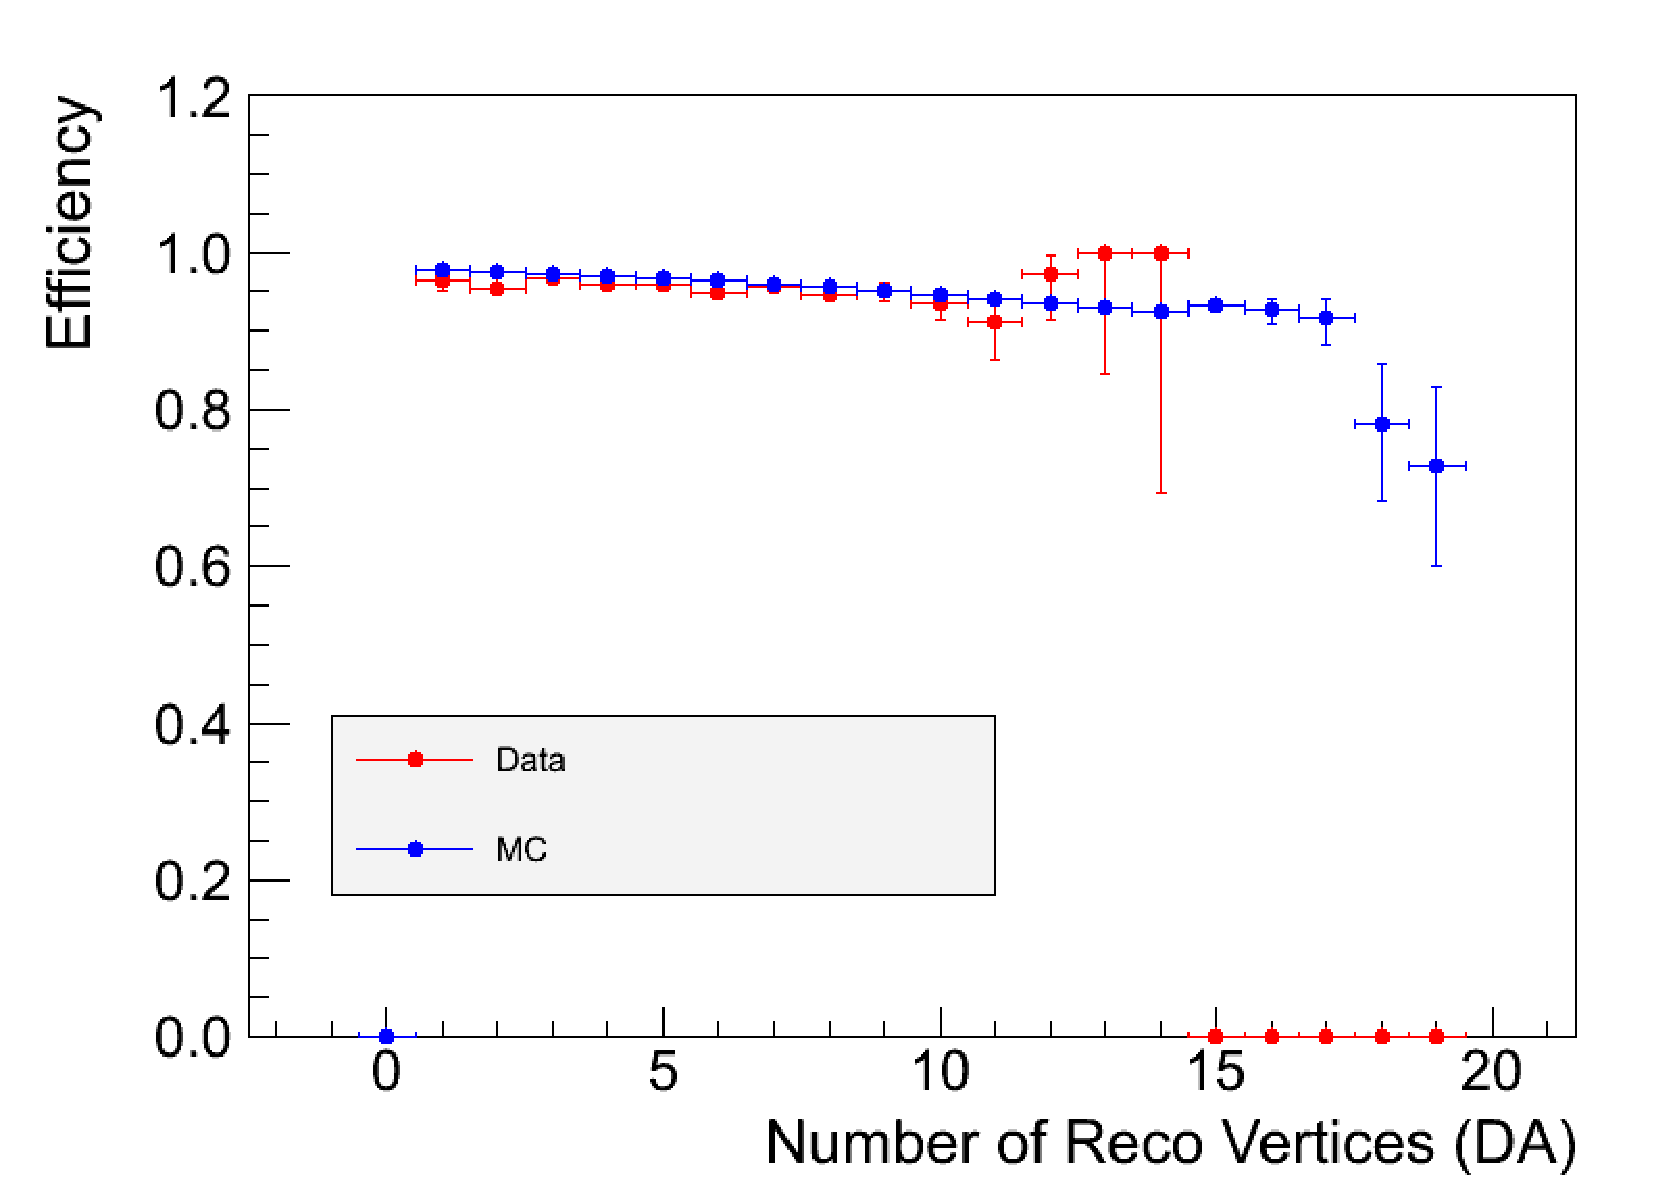
\includegraphics[width=0.45\textwidth]{figures/ElectronIsolationBarrelEffVsNVertices_TagAndProbe.pdf}}
\subfigure[Endcap]{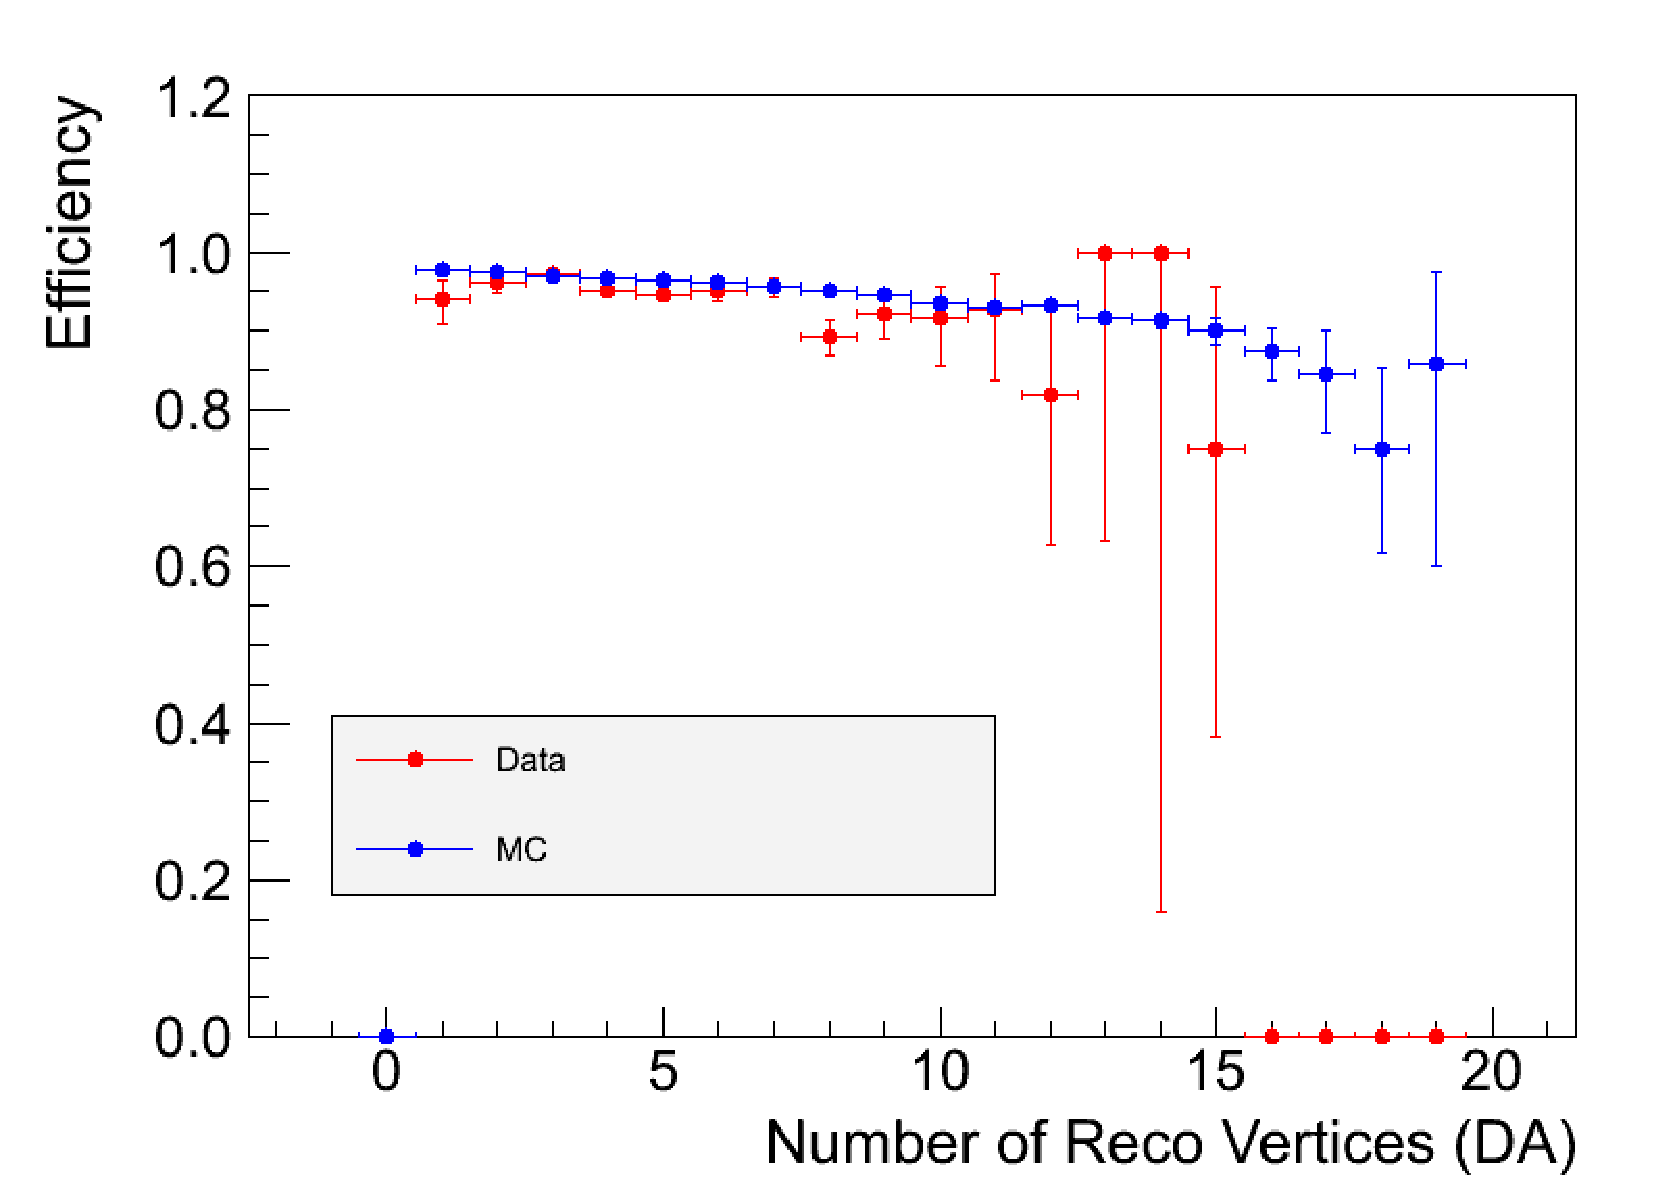
\includegraphics[width=0.45\textwidth]{figures/ElectronIsolationEndcapEffVsNVertices_TagAndProbe.pdf}}
\caption{Isolation efficiency vs number of reconstructed primary vertices for electrons, comparing the 
results from the tag and probe selection on 2011 data with the Z Monte Carlo simulation.}
\label{fig:eleIsoEff_TagAndProbe_vs_NVertices}
\end{center}
\end{figure}

\begin{figure}[!htbp]
\begin{center}
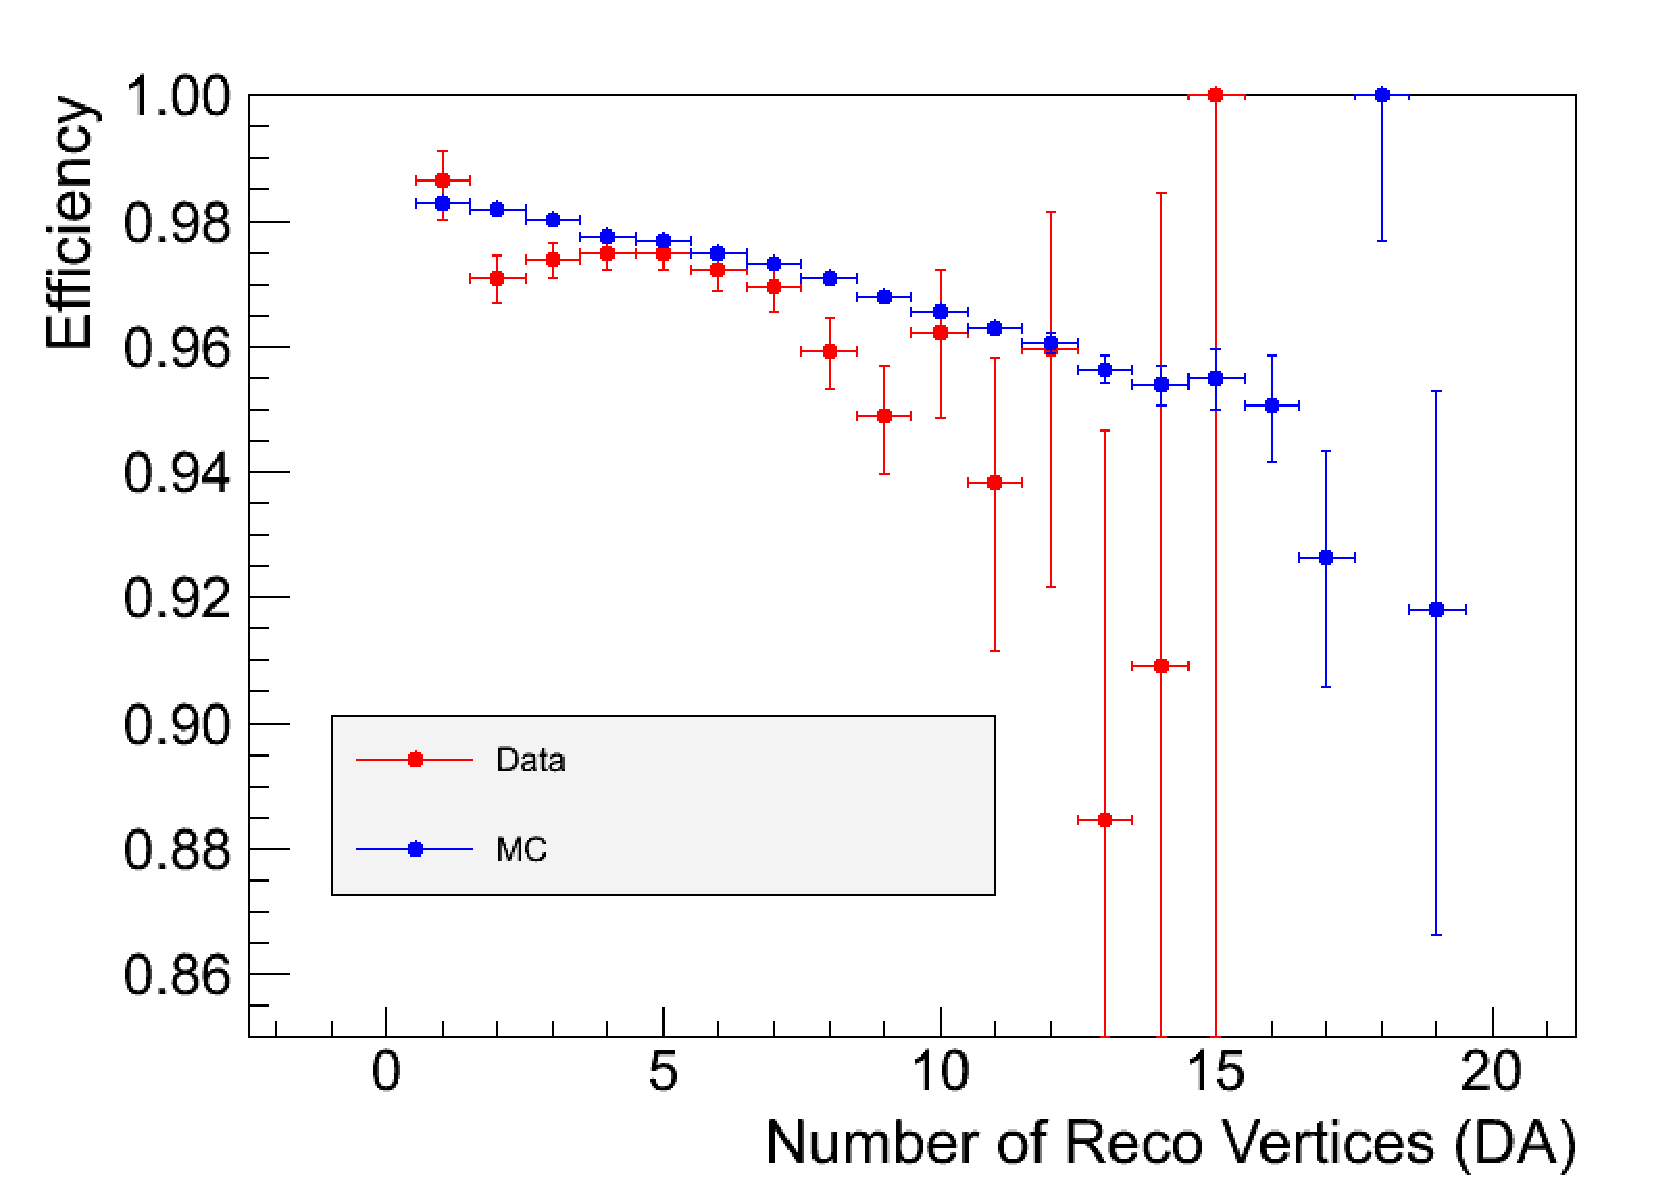
\includegraphics[width=0.45\textwidth]{figures/MuonIsolationEffVsNVertices_TagAndProbe.pdf}
\caption{Isolation efficiency vs number of reconstructed primary vertices for muons, comparing the 
results from the tag and probe selection on 2011 data with the Z Monte Carlo simulation.}
\label{fig:muIsoEff_TagAndProbe_vs_NVertices}
\end{center}
\end{figure}

Figs. \ref{fig:eleIsoEff_TagAndProbe_vs_NVertices} and \ref{fig:muIsoEff_TagAndProbe_vs_NVertices} 
show the isolation efficiency for electrons and muons respectively, measured using the
tag and probe selection, for 2011 data and Z Monte Carlo simulation. Agreement in these
efficiencies allow us to use the signal Monte Carlo to infer the efficiency loss under 
high pileup environment. The lepton isolation efficiency for HWW signal events are plotted
in Fig \ref{fig:HWW130IsoEff_vs_NVertices}, showing a loss of efficiency of 5\% for 
electrons and 2\% for muons, between events with one reconstructed primary vertex
and 10 reconstructed primary vertices. The efficiency loss for leptons with $p_{T}$ 
between $10$ and $20$ GeV is much larger compared to the efficiency loss for higher
$p_{T}$ leptons. As a result the efficiency loss on signal events is dependent 
on the mass of the Higgs boson. For a signal with Higgs mass of $130$ GeV, 
the average loss of efficiency for electrons and muons with $p_{T}>20$ GeV is
$2\%$ and $1\%$ respectively. 


\begin{figure}[!htbp]
\begin{center}
\subfigure[HWW130 Electrons]{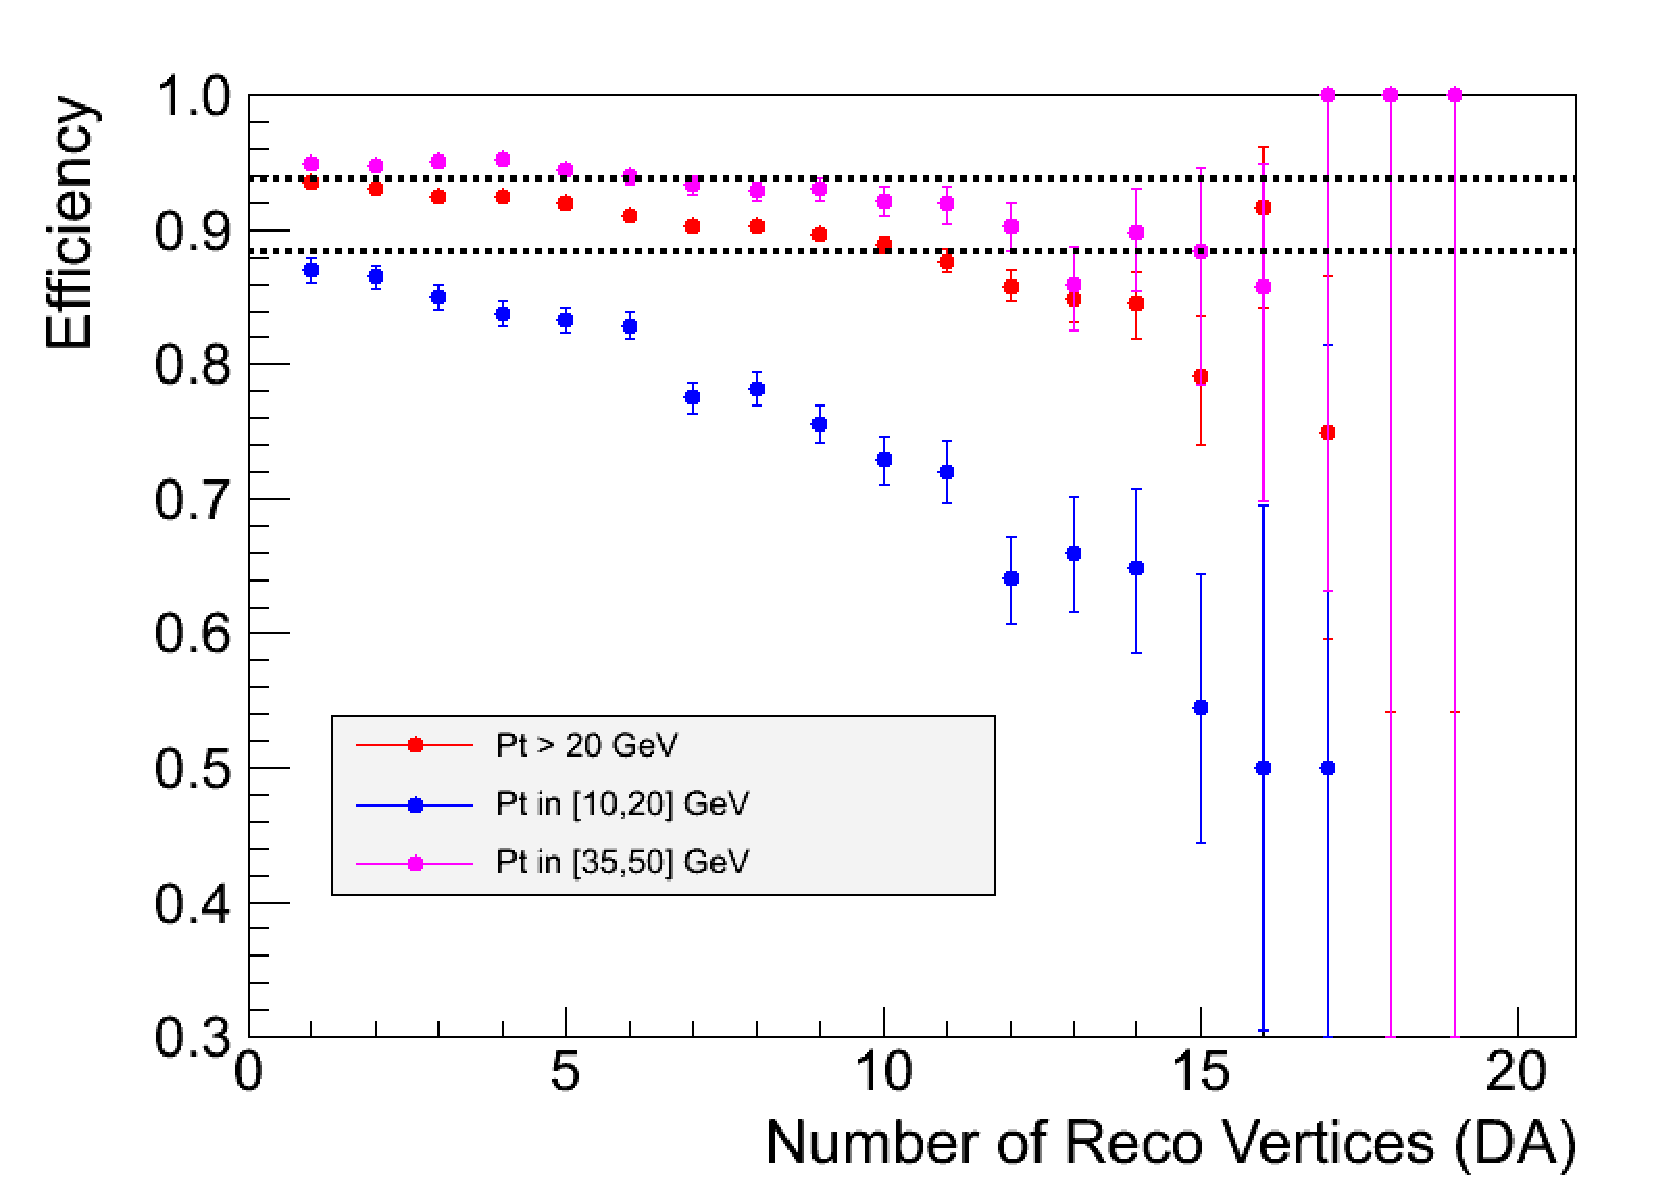
\includegraphics[width=0.45\textwidth]{figures/ElectronIsolationVsNVertices_HWW130.pdf}}
\subfigure[HWW130 Muons]{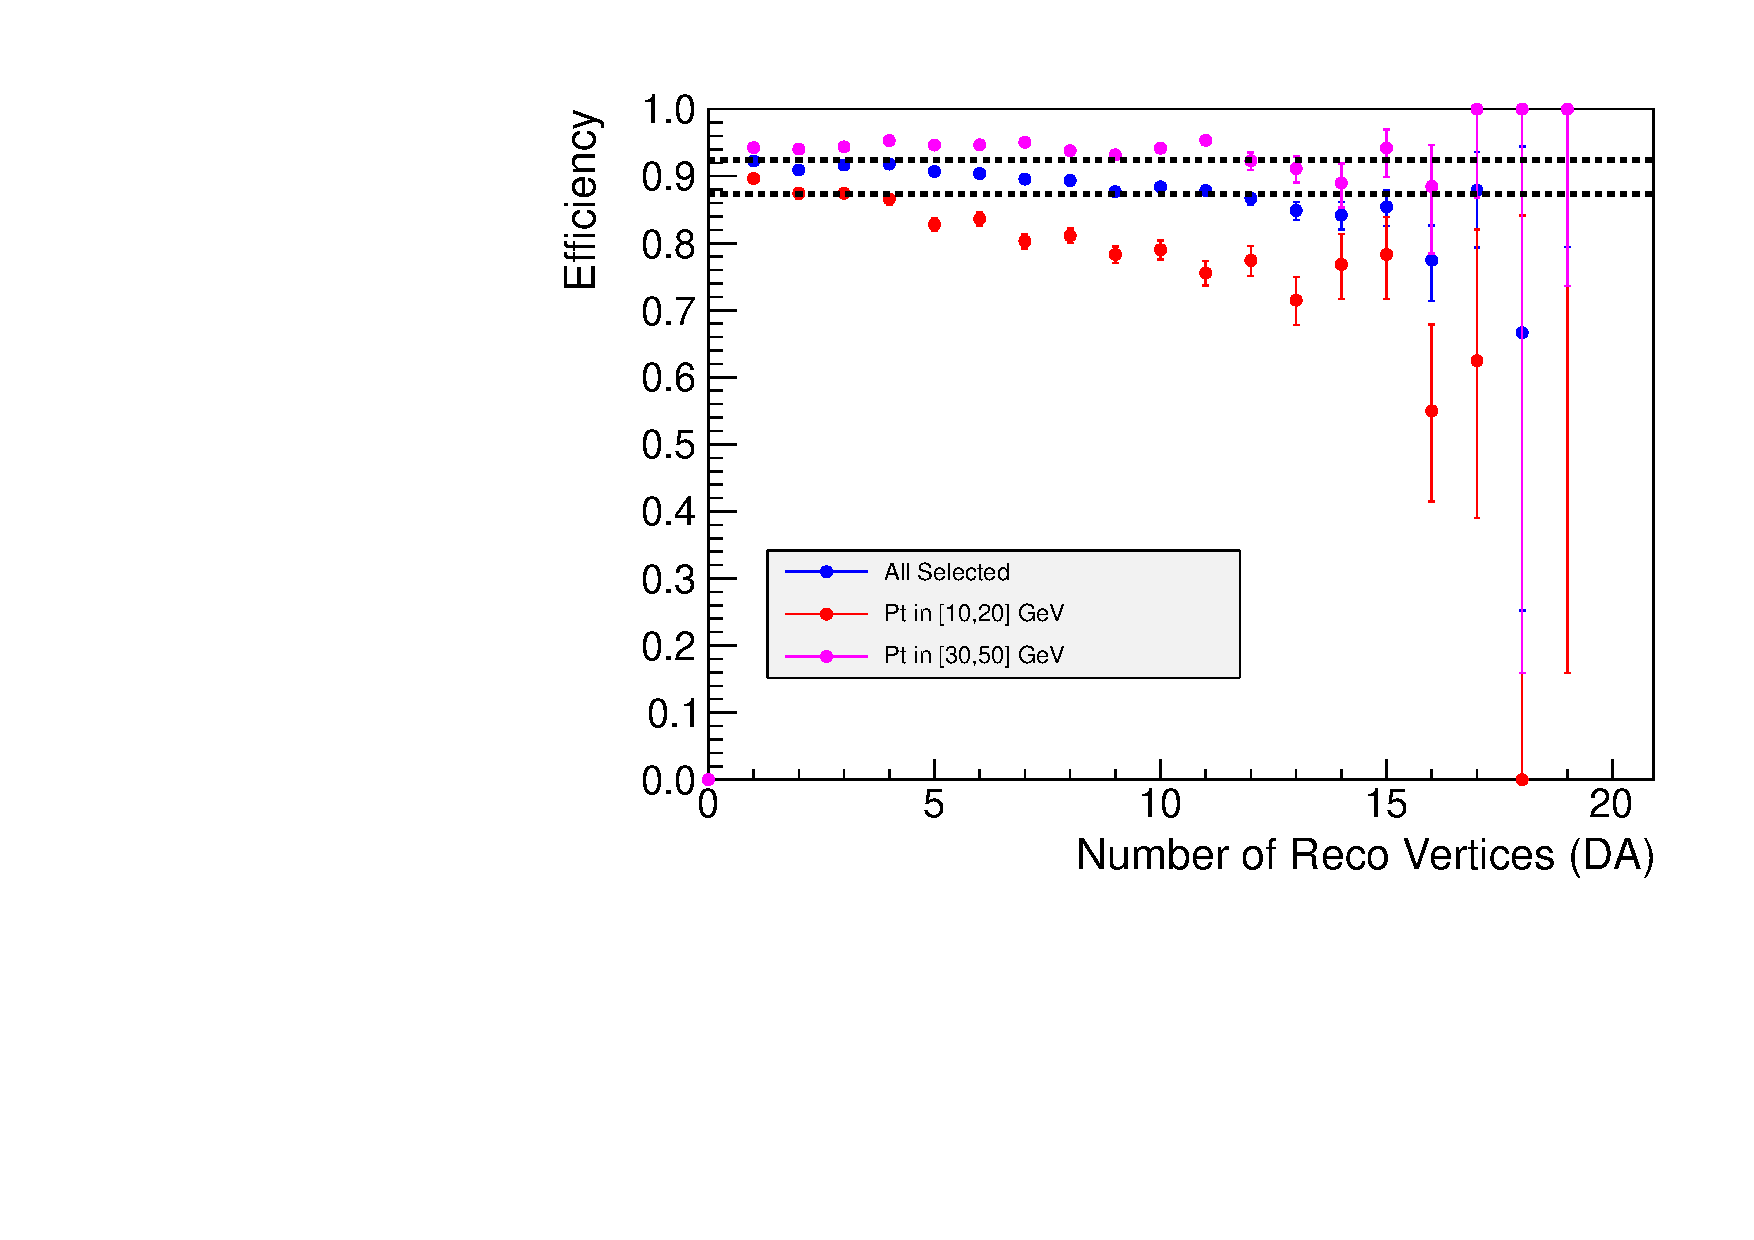
\includegraphics[width=0.45\textwidth]{figures/MuonIsolationVsNVertices_HWW130.pdf}}
\caption{Isolation efficiency vs number of reconstructed primary vertices for electrons and muons
in the HWW ($m_{H} = 130$) Monte Carlo simulation. The isolation efficiency for various $p_{T}$ 
bins are shown.}
\label{fig:HWW130IsoEff_vs_NVertices}
\end{center}
\end{figure}





\subsection{Mitigating the effect of Pileup}

Typical strategies for mitigating the effect of pileup on lepton isolation include
performing appropriate isolation energy corrections to recover inefficiencies, or 
parameterizing and re-tuning the cuts as a function of some observable correlated
to pileup. As a preliminary attempt at pileup corrections for isolation, we investigated
the possiblity to use the fastjet correction described in Section \ref{sec:sel_jets} 
assuming a fixed area corresponding to the isolation cone of $\Delta$R $< 0.3$. 
The isolation efficiency for electrons and muons from HWW signal events are shown in 
Figure \ref{fig:HWW130IsoEff_vs_NVertices_FastjetCorrection}, comparing
the fastjet corrected isolation with the uncorrected isolation as a function of the 
number of reconstructed primary vertices. We observe that the efficiency does indeed become 
flat for signal. However, we observe that for the background leptons, this correction appears
over-correct the pileup contribution, demonstrated by the fact that the efficiency increases
as a function of the number of reconstructed primary vertices shown in Fig 
\ref{fig:BkgIsoEff_vs_NVertices_FastjetCorrection}. 


\begin{figure}[!htbp]
\begin{center}
\subfigure[HWW130 Electrons]{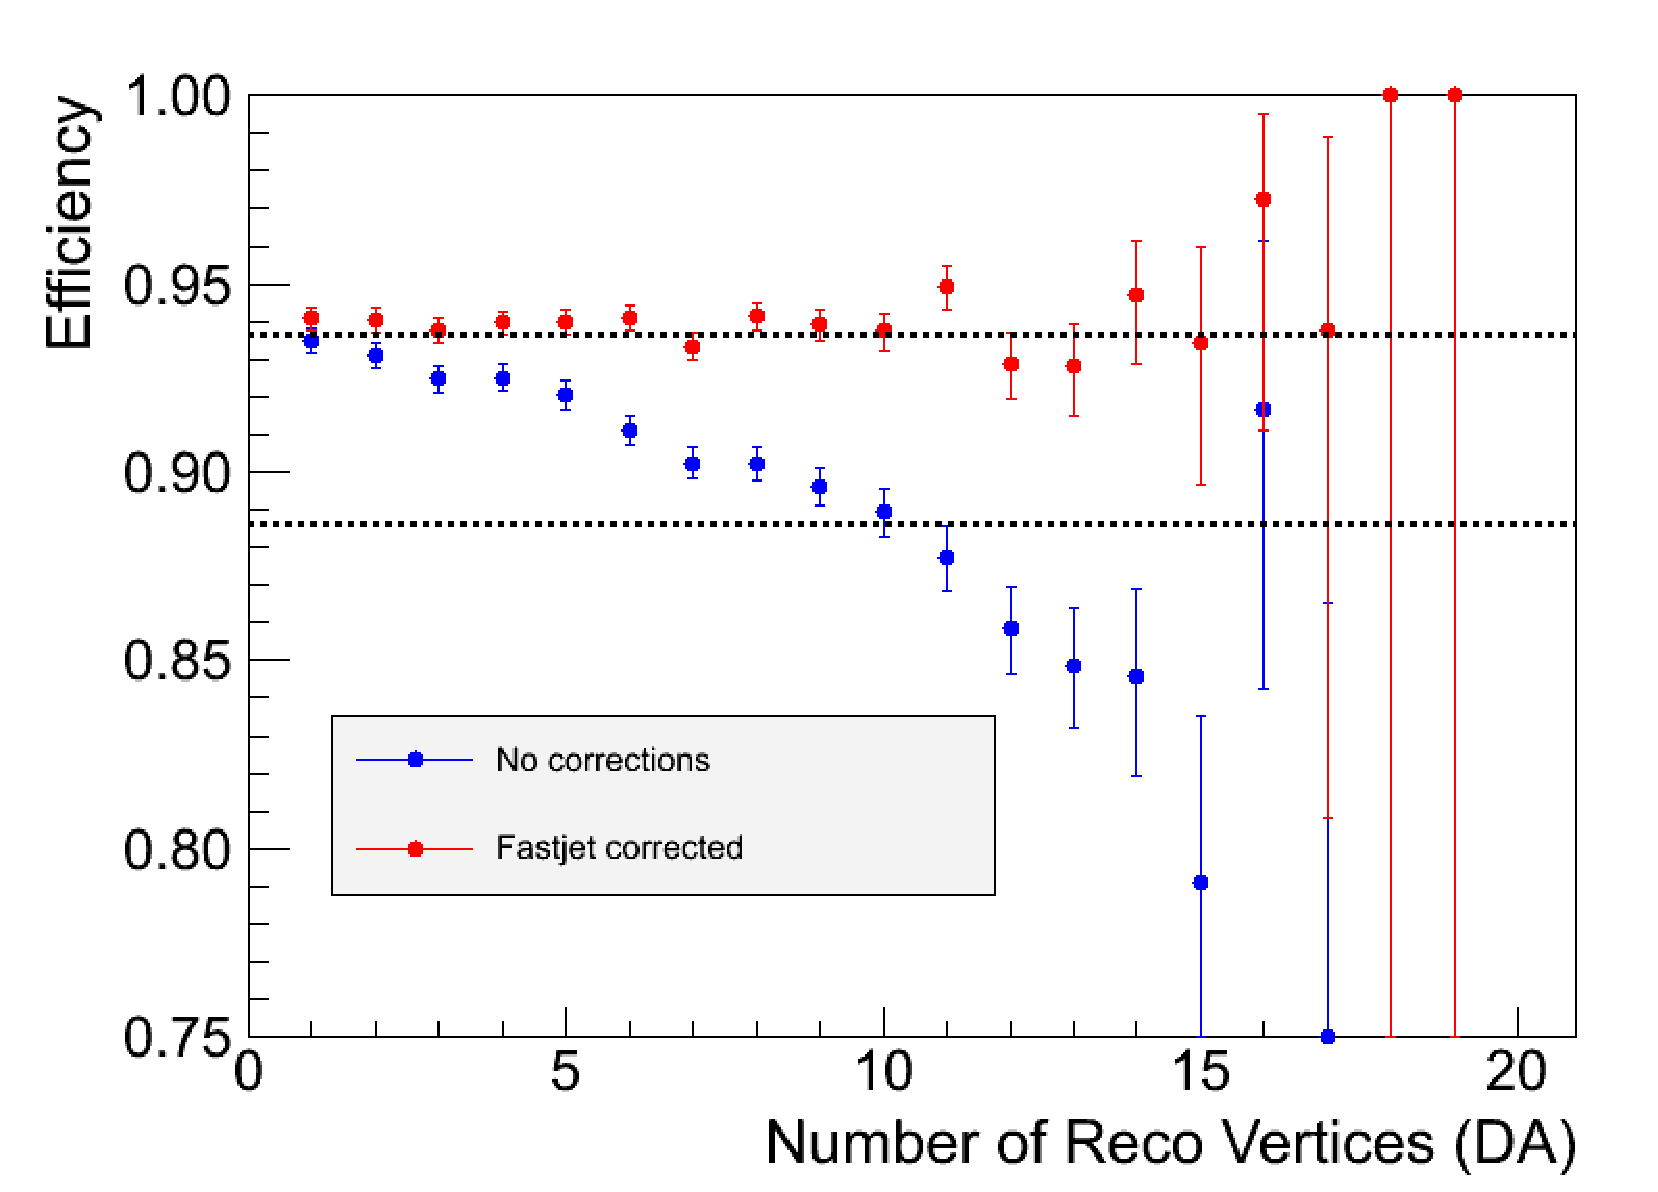
\includegraphics[width=0.45\textwidth]{figures/ElectronIsolationVsNVertices_HWW130_FastjetCorrection.pdf}}
\subfigure[HWW130 Muons]{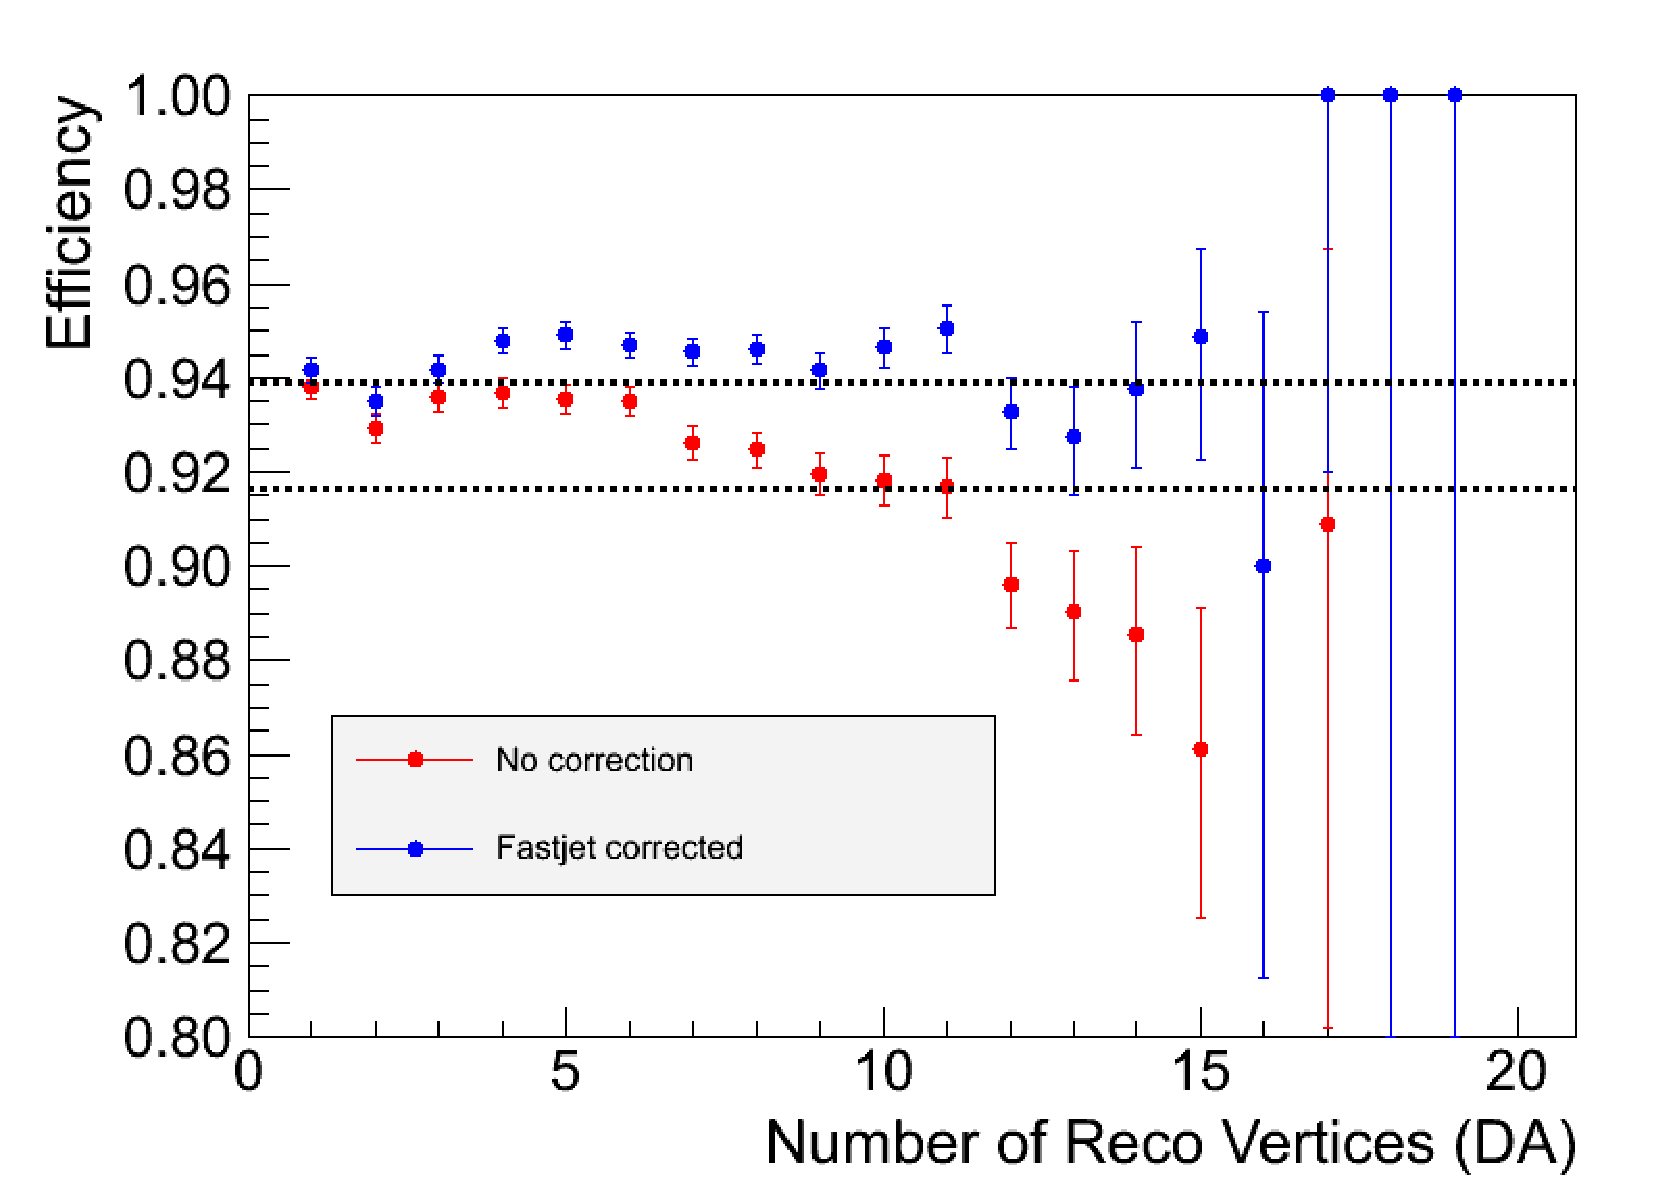
\includegraphics[width=0.45\textwidth]{figures/MuonIsolationVsNVertices_HWW130_FastjetCorrection.pdf}}
\caption{Signal lepton isolation efficiency vs number of reconstructed primary vertices, comparing uncorrected 
and fastjet corrected isolation cuts in the HWW ($m_{H} = 130$) Monte Carlo simulation. Leptons
with $p_{T} > 20$ GeV are used.}
\label{fig:HWW130IsoEff_vs_NVertices_FastjetCorrection}
\end{center}
\end{figure}

\begin{figure}[!htbp]
\begin{center}
\subfigure[Fake rate Data]{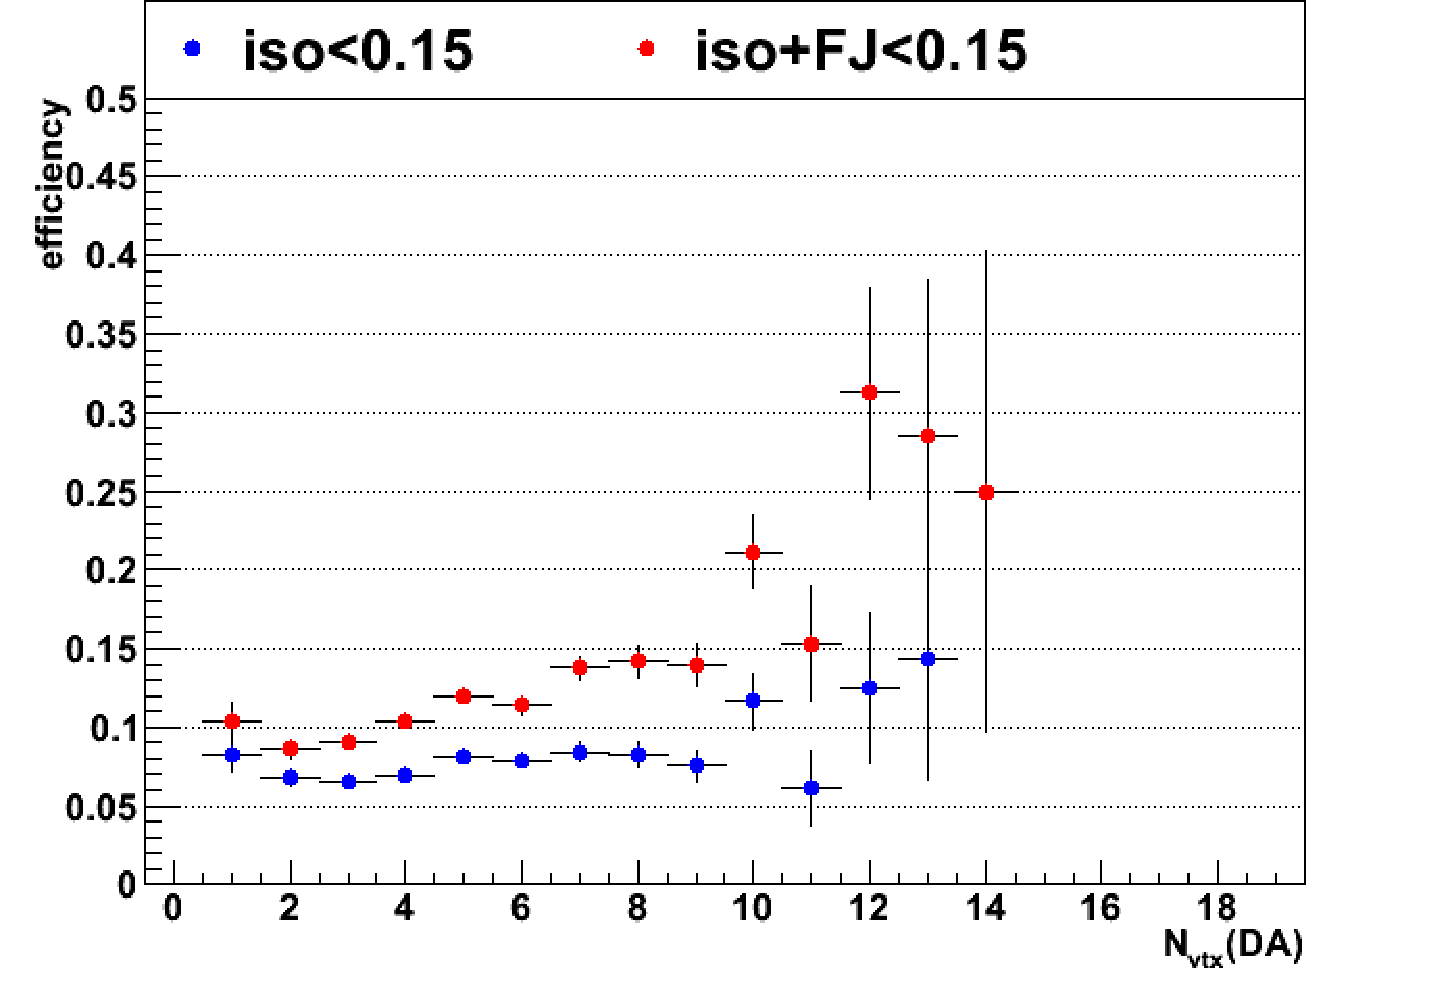
\includegraphics[width=0.45\textwidth]{figures/MuonIsolationVsNVertices_JetData_FastjetCorrection.pdf}}
\subfigure[QCD MC]{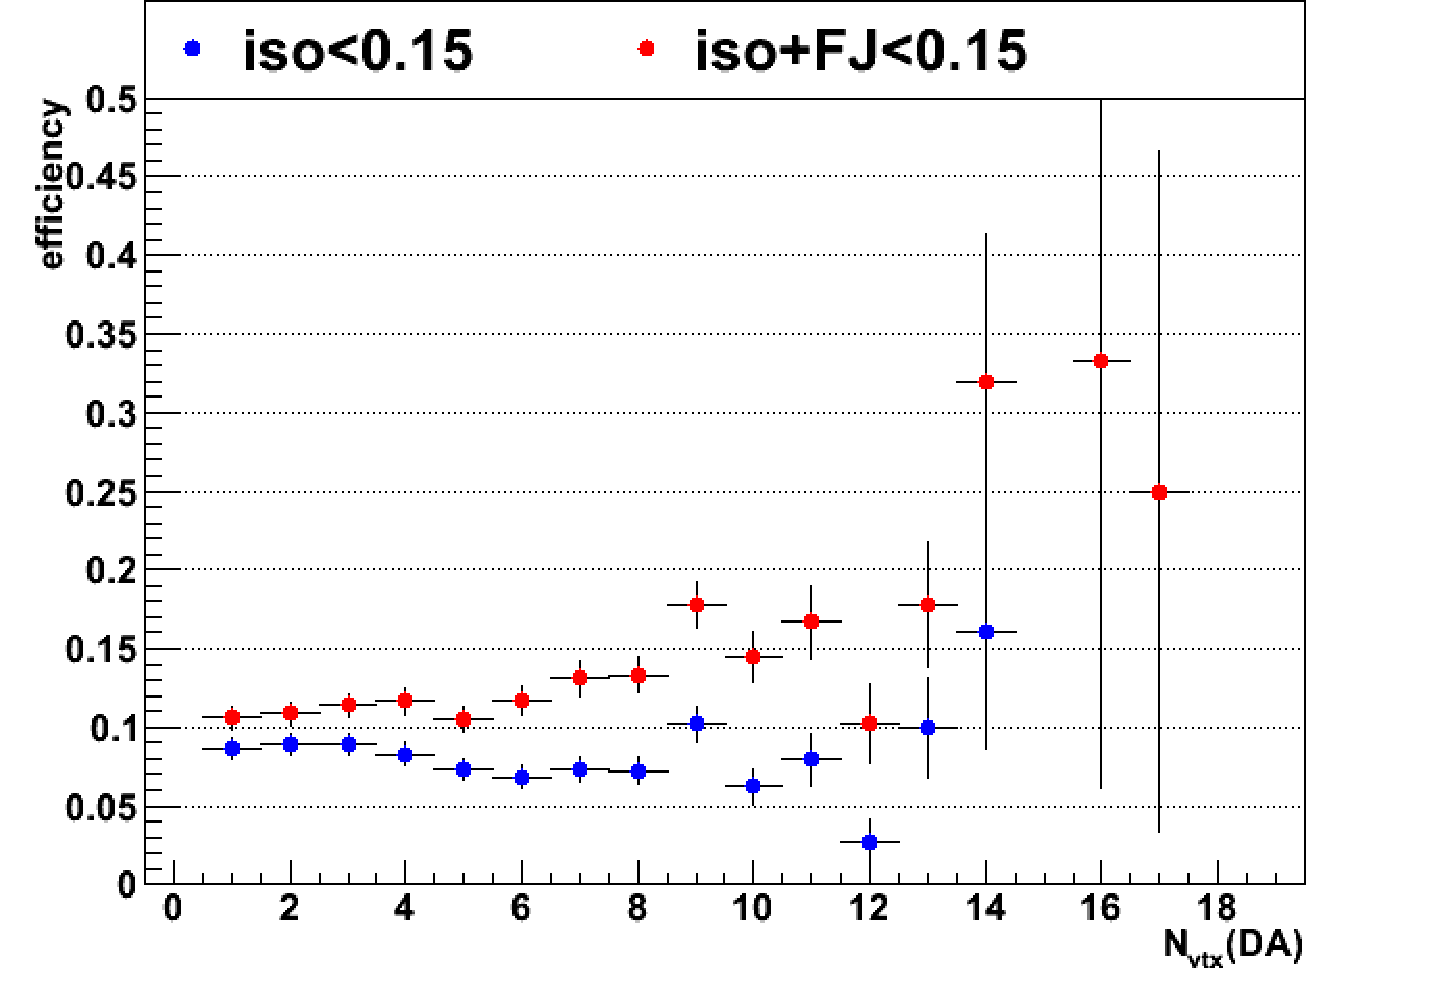
\includegraphics[width=0.45\textwidth]{figures/MuonIsolationVsNVertices_QCDMC_FastjetCorrection.pdf}}
\caption{Background lepton isolation efficiency vs number of reconstructed primary vertices, comparing uncorrected 
and fastjet corrected isolation cuts. Results for a fake lepton dominated data sample, and the QCD Monte Carlo simulation
are shown. }
\label{fig:BkgIsoEff_vs_NVertices_FastjetCorrection}
\end{center}
\end{figure}

One possible explanation for this behavior is that it is due to the inconsistency of applying
a particle flow based energy density calculation to a detector based isolation quantity. Therefore,
we study the use of a particle flow based isolation quantity. For electrons, in order to 
remove any remaining footprint, we veto any neutral hadron particle flow objects with
$\Delta$R $ < 0.07$ corresponding to the size of one calorimeter tower , and we 
veto any particle flow photons or particle flow electrons inside of the $\eta$-strip defined by
$|\Delta\eta| < 0.025$ in order to remove the effect of unrecovered bremstrahlung. No such
footprint removal is necessary for muons.


\subsubsection{Association of charged particles to the primary vertex}

The first handle to address pileup subtraction is to apply a cut in $\Delta$z for 
charged particles or tracks. Figure \ref{fig:IsoPerformance_EleBarrel_dZCut} shows the difference
in performance between rejecting charged particles inside the isolation cone 
incompatible with the primary vertex and not rejecting them. There is a clear increase
in performance if one requires this rejection.

\begin{figure}[!htbp]
\begin{center}
\subfigure[NVtx: 3-6]{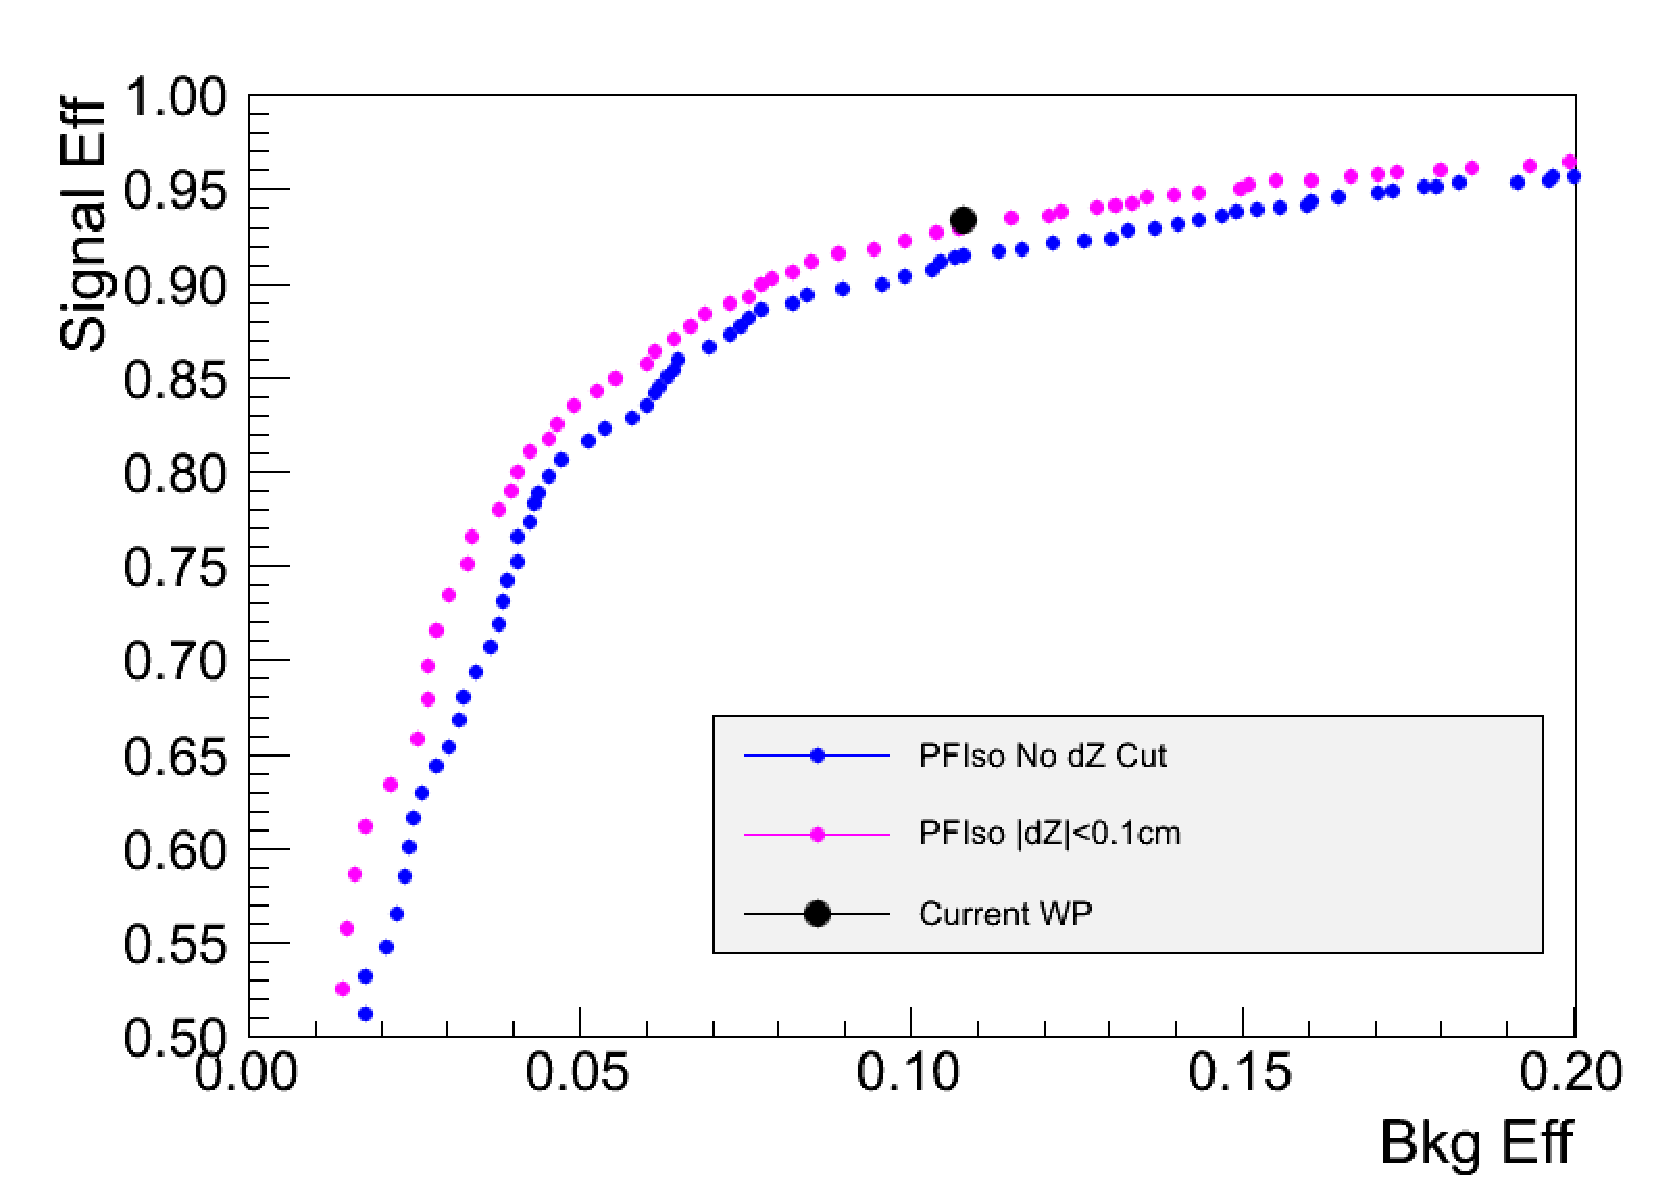
\includegraphics[width=0.48\textwidth]{figures/IsoPerformance_EleBarrel_NVtx3to6_dZCut_Pt20To30.pdf}}
\subfigure[NVtx: 7-15]{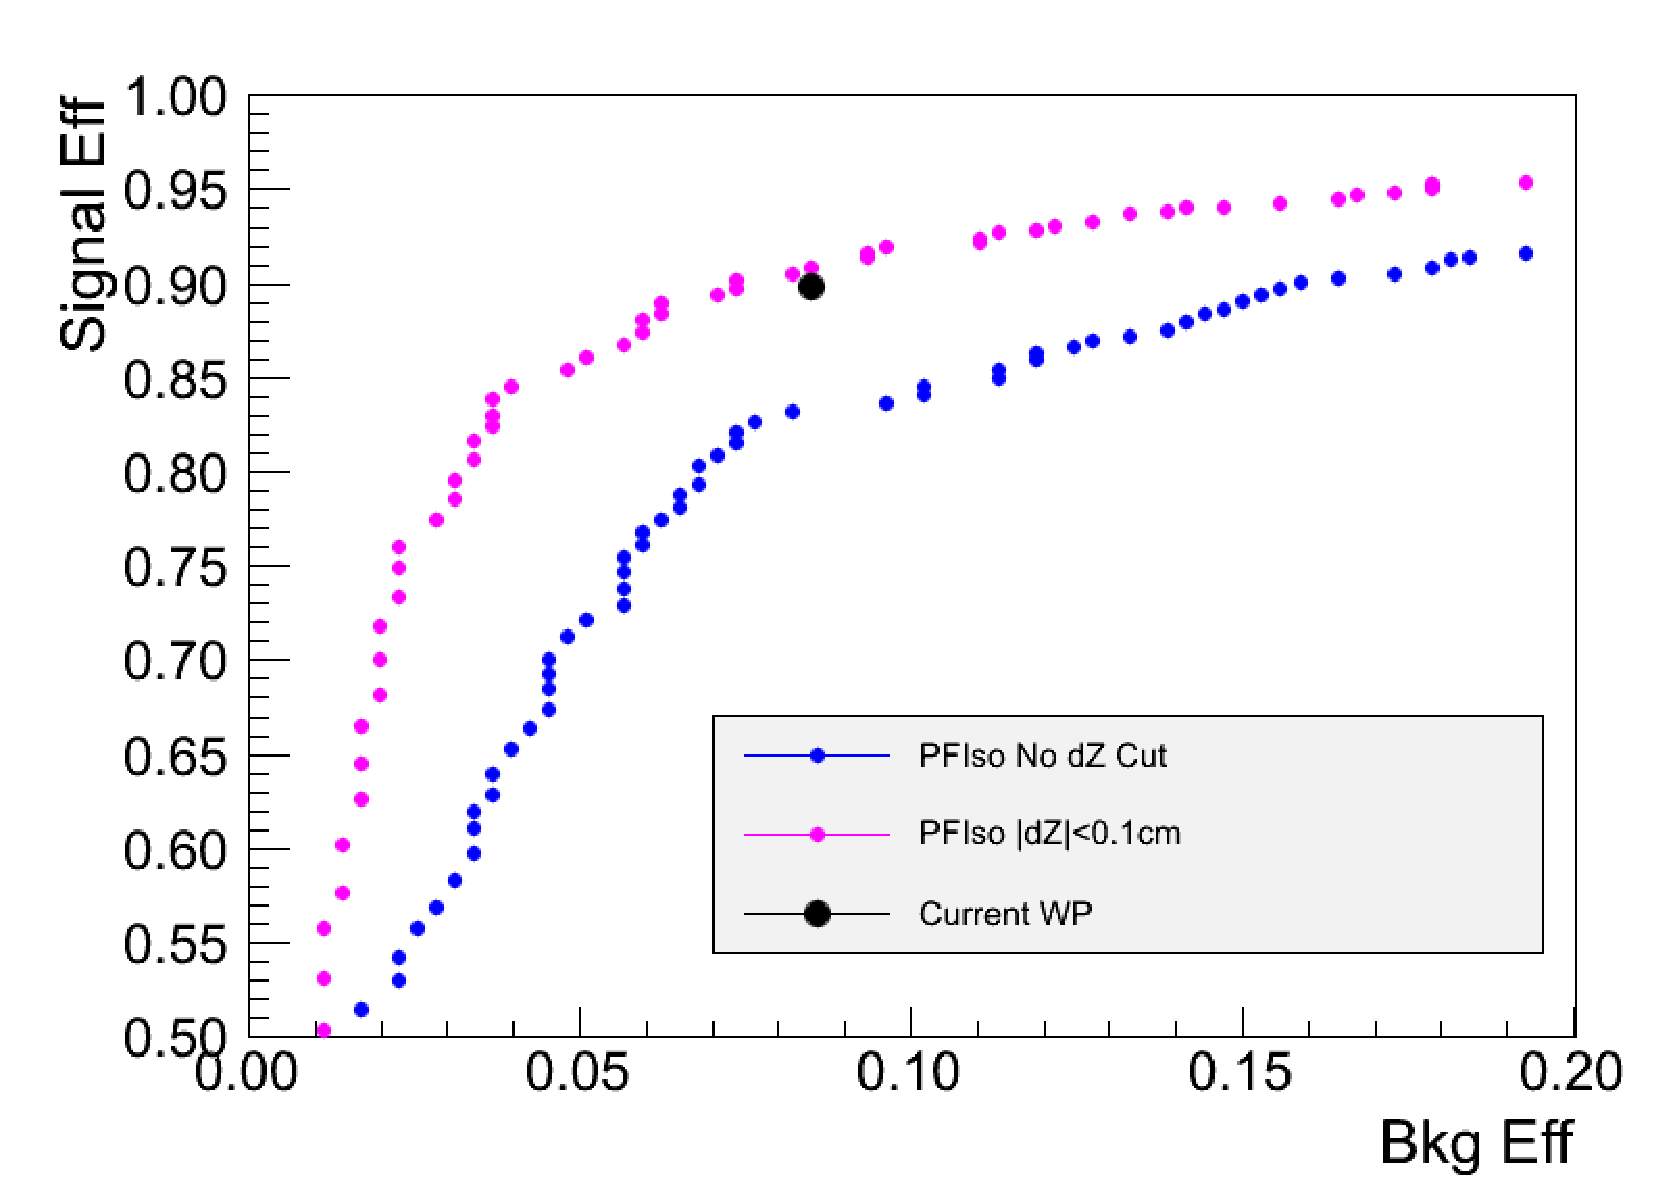
\includegraphics[width=0.48\textwidth]{figures/IsoPerformance_EleBarrel_NVtx7to15_dZCut_Pt20To30.pdf}}
\caption{ Signal efficiency (HWW130) vs background efficiency for barrel electrons separated into 
low and high pileup, comparing with and without the $\Delta$z requirement for charged particles.
Electrons with $p_{T} > 20$ GeV are used. }
\label{fig:IsoPerformance_EleBarrel_dZCut}
\end{center}
\end{figure}


\subsubsection{Event Energy Density based Corrections}
\label{sec:CorrectionBasedIsolation}

Having rejected charged particles from pileup interactions in the isolation cone, there are
a couple of ways to reject neutral particles from pileup. One scheme is to perform a 
subtraction of energy inside the isolation cone due to pileup based on the average energy
density in the event. We first compute the average energy density, $\rho_{\mathrm{FJ}}$ due to 
pileup using either the Fast Jet procedure or the procedure employing a fixed grid of squares, 
plot the mean of $\rho_{\mathrm{FJ}}$ as a function of
the number of reconstructed vertices, and finally perform a linear fit. Next we perform the 
same linear fit in the mean of the relevant isolation variable as a function of the number of 
reconstructed vertices, and then define the effective area as 
$\mathrm{EA} = \mathrm{slope}_{\rho} / \mathrm{slope}_{\mathrm{iso}}$. This effective area 
is multiplied by the $\rho$ for every event to obtain the contamination of pileup energy
inside the isolation cone. This energy contamination is subtracted from the lepton isolation
to correct for pileup. Figure \ref{fig:IsoPerformance_EleBarrel_EffectiveAreaCorrection}
compares the performance of the standard isolation and the particle flow isolation with and
without the effective area corrections. We observe that there is essentially no change
in the performance after performing the correction procedure described above.

\begin{figure}[!htbp]
\begin{center}
\subfigure[$p_{T}$ in $(10,15)$ GeV]{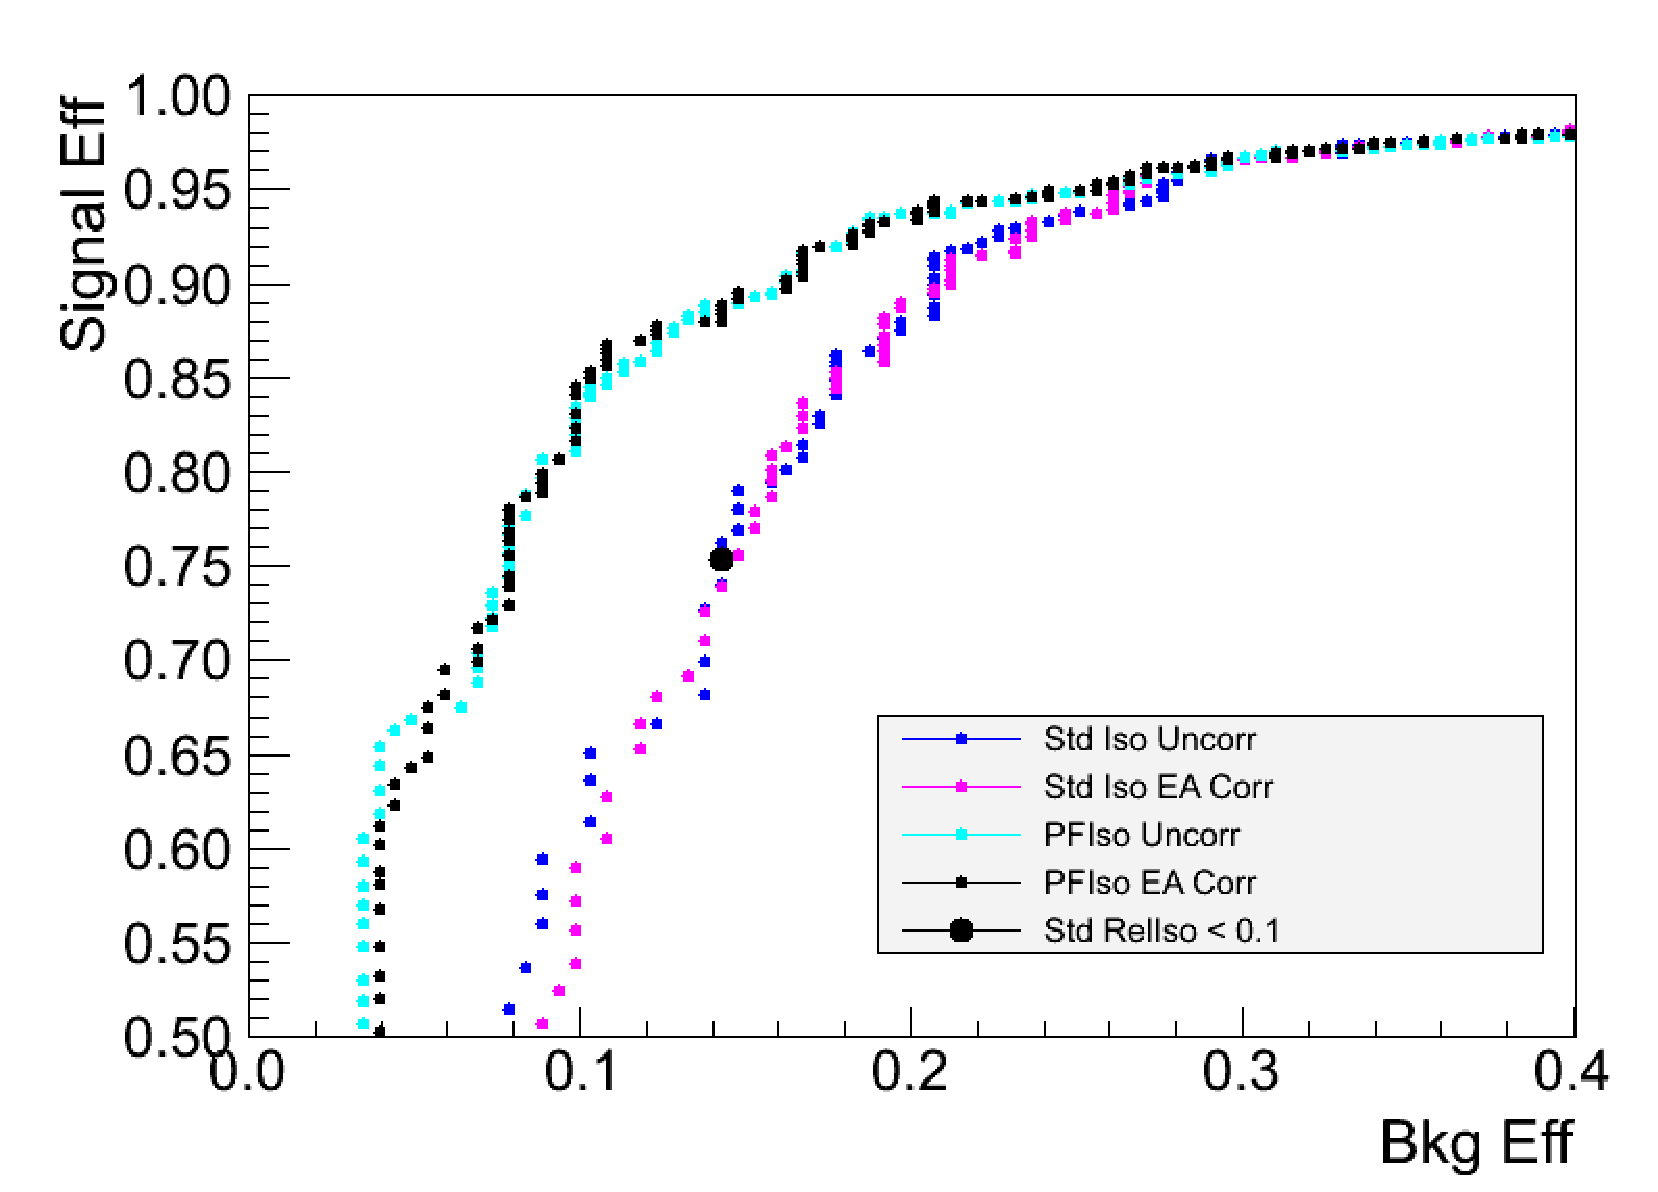
\includegraphics[width=0.48\textwidth]{figures/IsoPerformance_EleBarrel_EACorr_NVtx7To15_Pt10To15.pdf}}
\subfigure[$p_{T}$ in $(20,30)$ GeV]{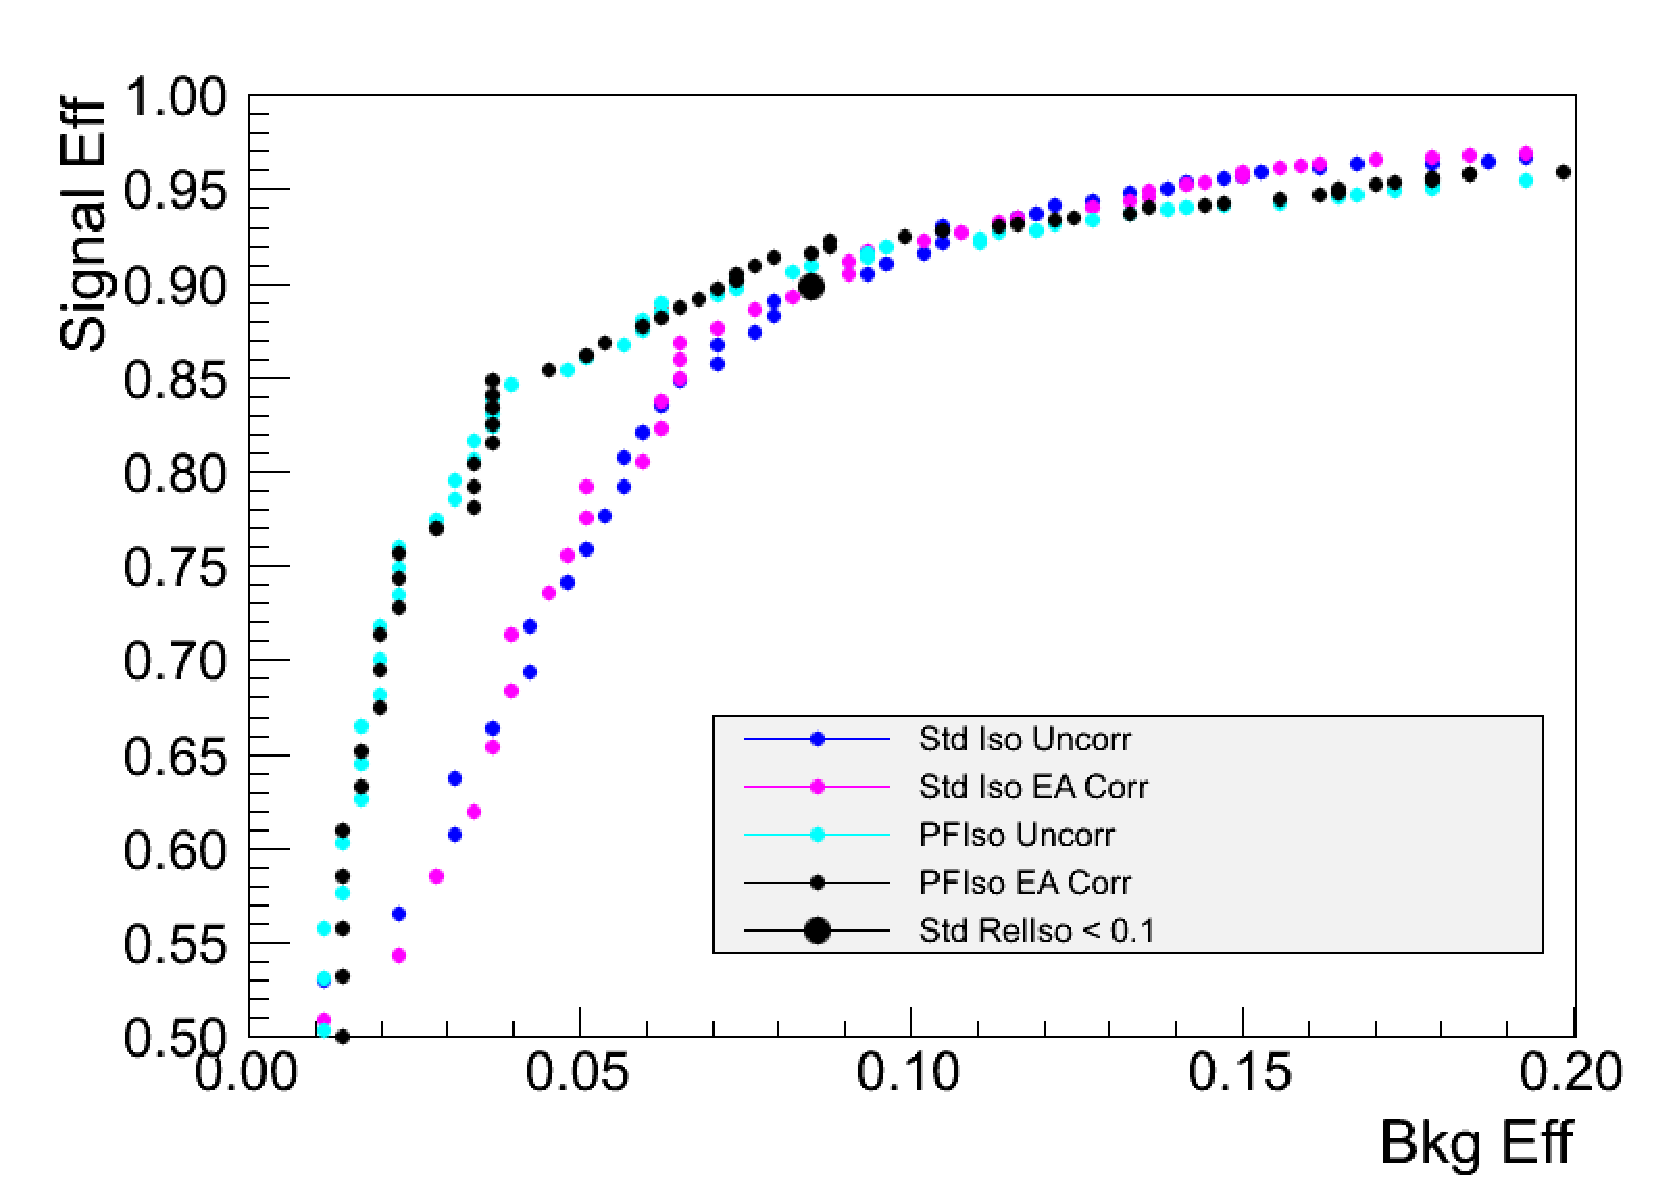
\includegraphics[width=0.48\textwidth]{figures/IsoPerformance_EleBarrel_EACorr_NVtx7To15_Pt20To30.pdf}}
\caption{Signal efficiency (HWW130) vs background efficiency for barrel electrons separated into 
low and high $p_{T}$ bins, comparing the effect of applying the effective area pileup correction.
The high pileup scenario (NVtx $7$-$15$) is shown.}
\label{fig:IsoPerformance_EleBarrel_EffectiveAreaCorrection}
\end{center}
\end{figure}


\subsubsection{Threshold-based Rejection of PU Contamination}
\label{sec:ThresholdBasedIsolation}
An alternative scheme for addressing pileup is to increase the $p_{T}$ threshold on neutral 
particles inside the isolation cone. Since particles produced in typical pileup events are
fairly low in $p_{T}$, this decreases sensitivity of the isolation cut to the presence of 
pileup. In Figure \ref{fig:IsoPerformance_Ele_PtThresholds}, we compare the performance
of the particle flow isolation cut, varying the $p_{T}$ threshold for neutral particles
inside the isolation cone. We observe a fairly small degradation in performance going up
to a threshold of $1.0$ GeV. In the endcap, the degradation in performance is a bit
larger, but acceptable. 

\begin{figure}[!htbp]
\begin{center}
\subfigure[Barrel]{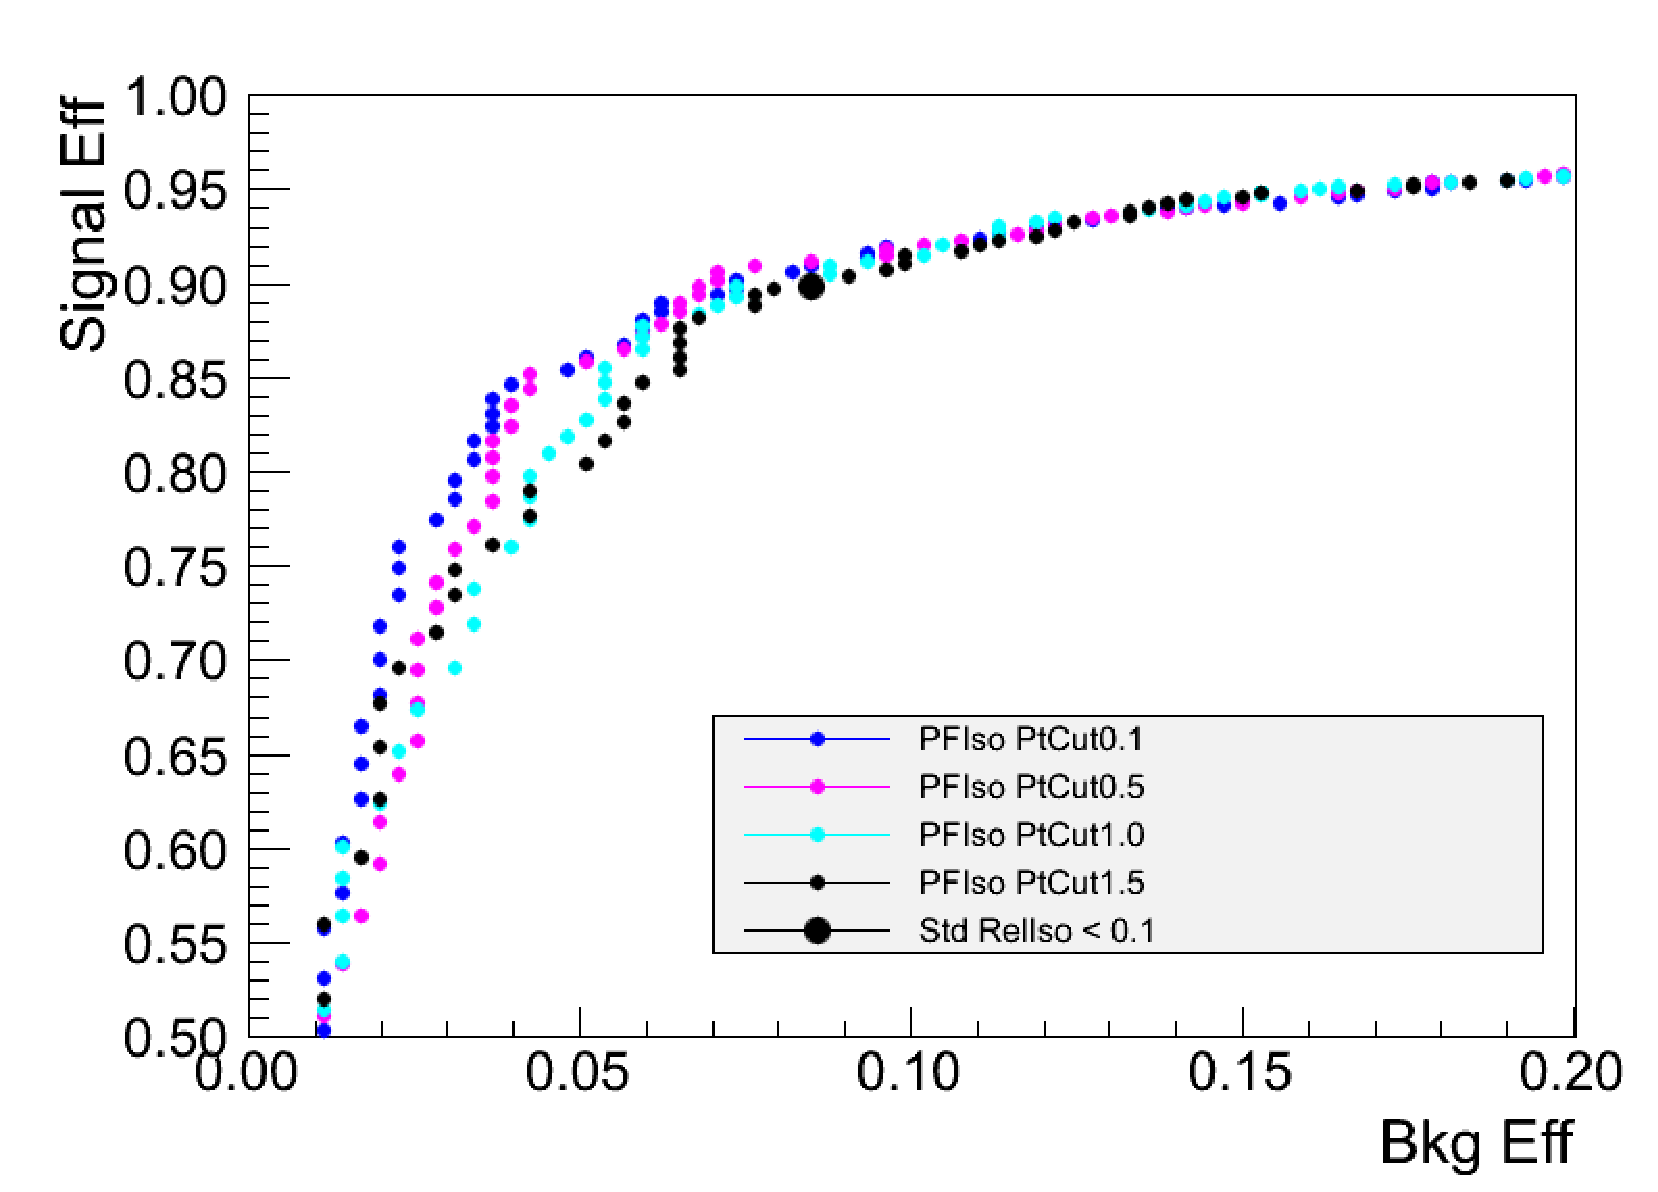
\includegraphics[width=0.48\textwidth]{figures/IsoPerformance_EleBarrel_PtThreshold_NVtx7To15_Pt20To30.pdf}}
\subfigure[Endcap]{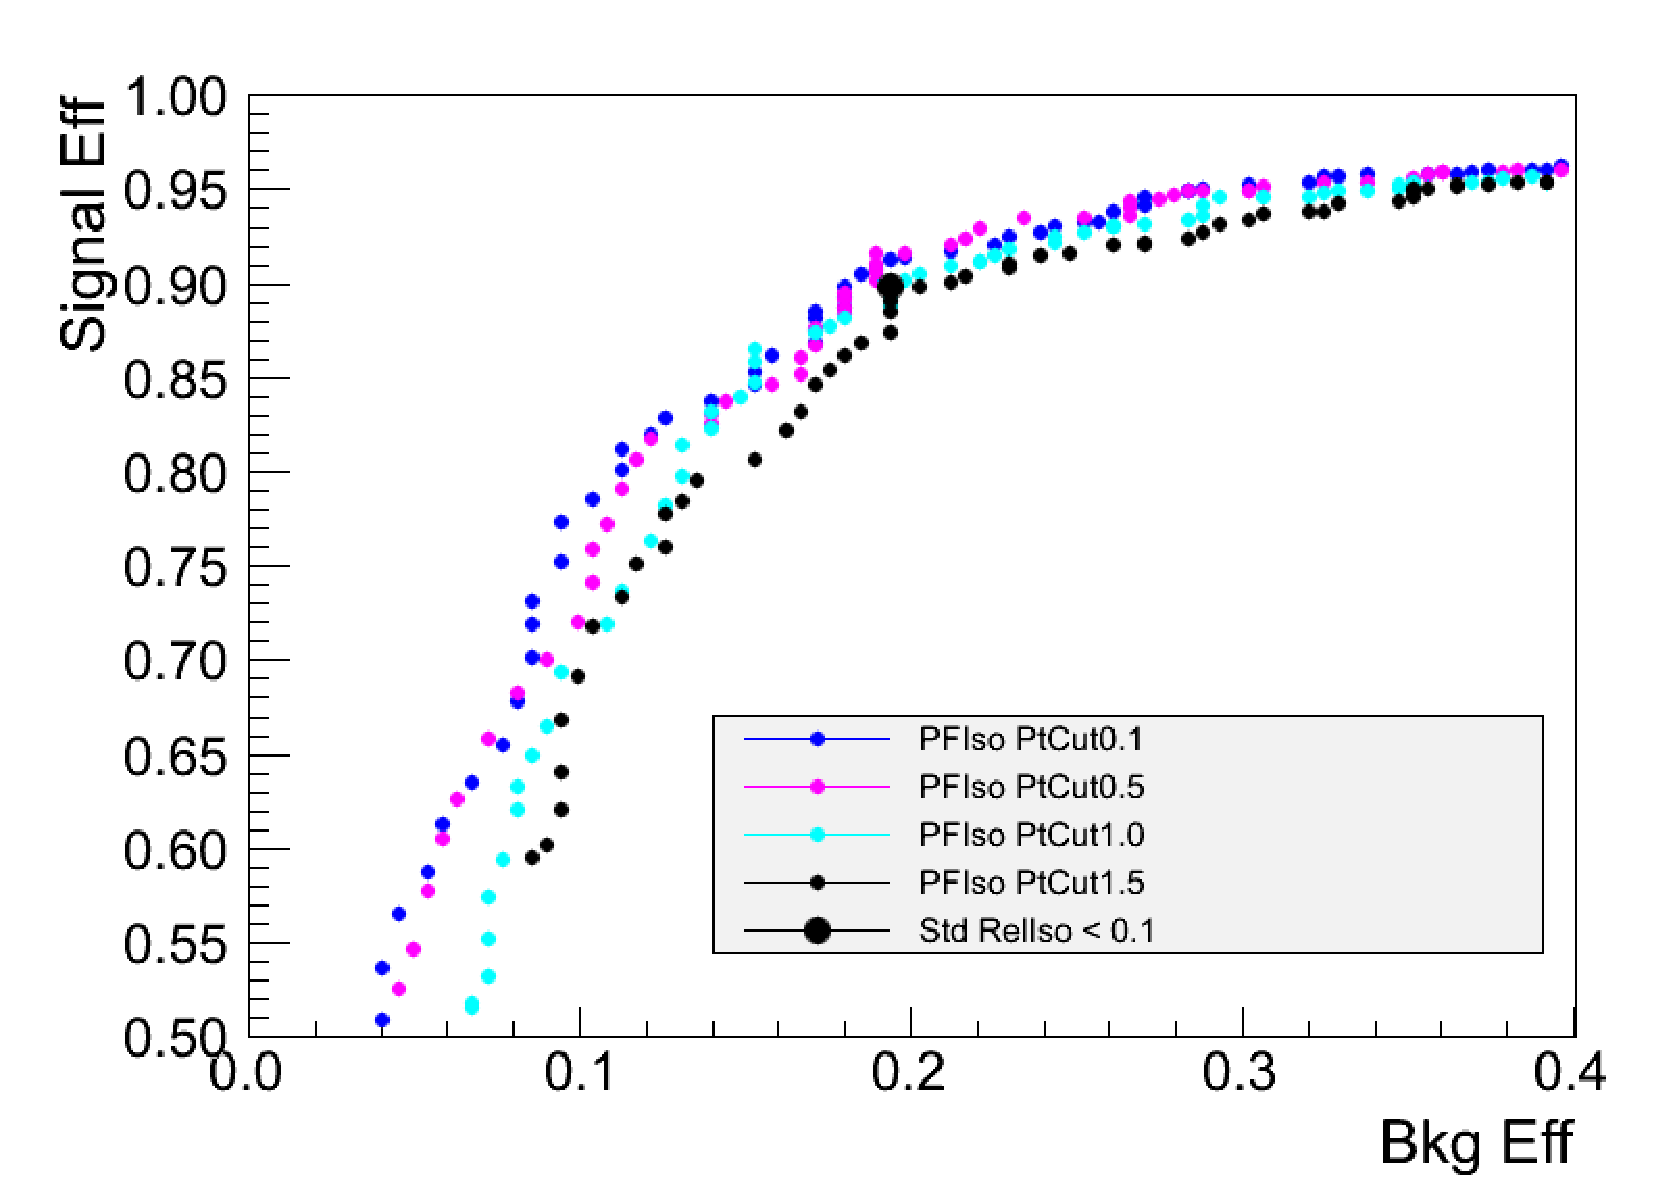
\includegraphics[width=0.48\textwidth]{figures/IsoPerformance_EleEndcap_PtThreshold_NVtx7To15_Pt20To30.pdf}}
\caption{Signal efficiency (HWW130) vs background efficiency for electrons with $p_{T}$ between $20$ and $30$ GeV
separated into barrel and endcap, comparing the effect of applying different $p_{T}$ thresholds on neutral particles.
The high pileup scenario (NVtx $7$-$15$) is shown.}
\label{fig:IsoPerformance_Ele_PtThresholds}
\end{center}
\end{figure}


To evaluate the effectiveness in mitigating the efficiency loss due to pileup, we study the isolation
efficiency as a function of the number of reconstructed vertices in the Higgs Monte Carlo simulation with a higgs 
mass of $130$ GeV. Figures \ref{fig:EleIsoEffVsNVtx_PFIso_Pt10To15} and \ref{fig:EleIsoEffVsNVtx_PFIso_Pt20To30}
show the decrease in efficiency with more pileup for low and high $p_{T}$ electrons respectively. In Table 
\ref{tab:EleIsoEfficiency_LossFromPileup_CompareStdWithPF}, we compare the efficiency loss from no pileup 
to $10$ reconstructed primary vertices for the standard detector based uncorrected isolation cut and the 
particle flow isolation cut with the $1$ GeV threshold on neutral particles. We observe a significant decrease
in the sensitivity of the isolation efficiency to the presence of pileup when we employ a $1GeV$ threshold on
the $p_{T}$ of the particle flow objects inside the isolation cone.

\begin{figure}[!htbp]
\begin{center}
\subfigure[Barrel]{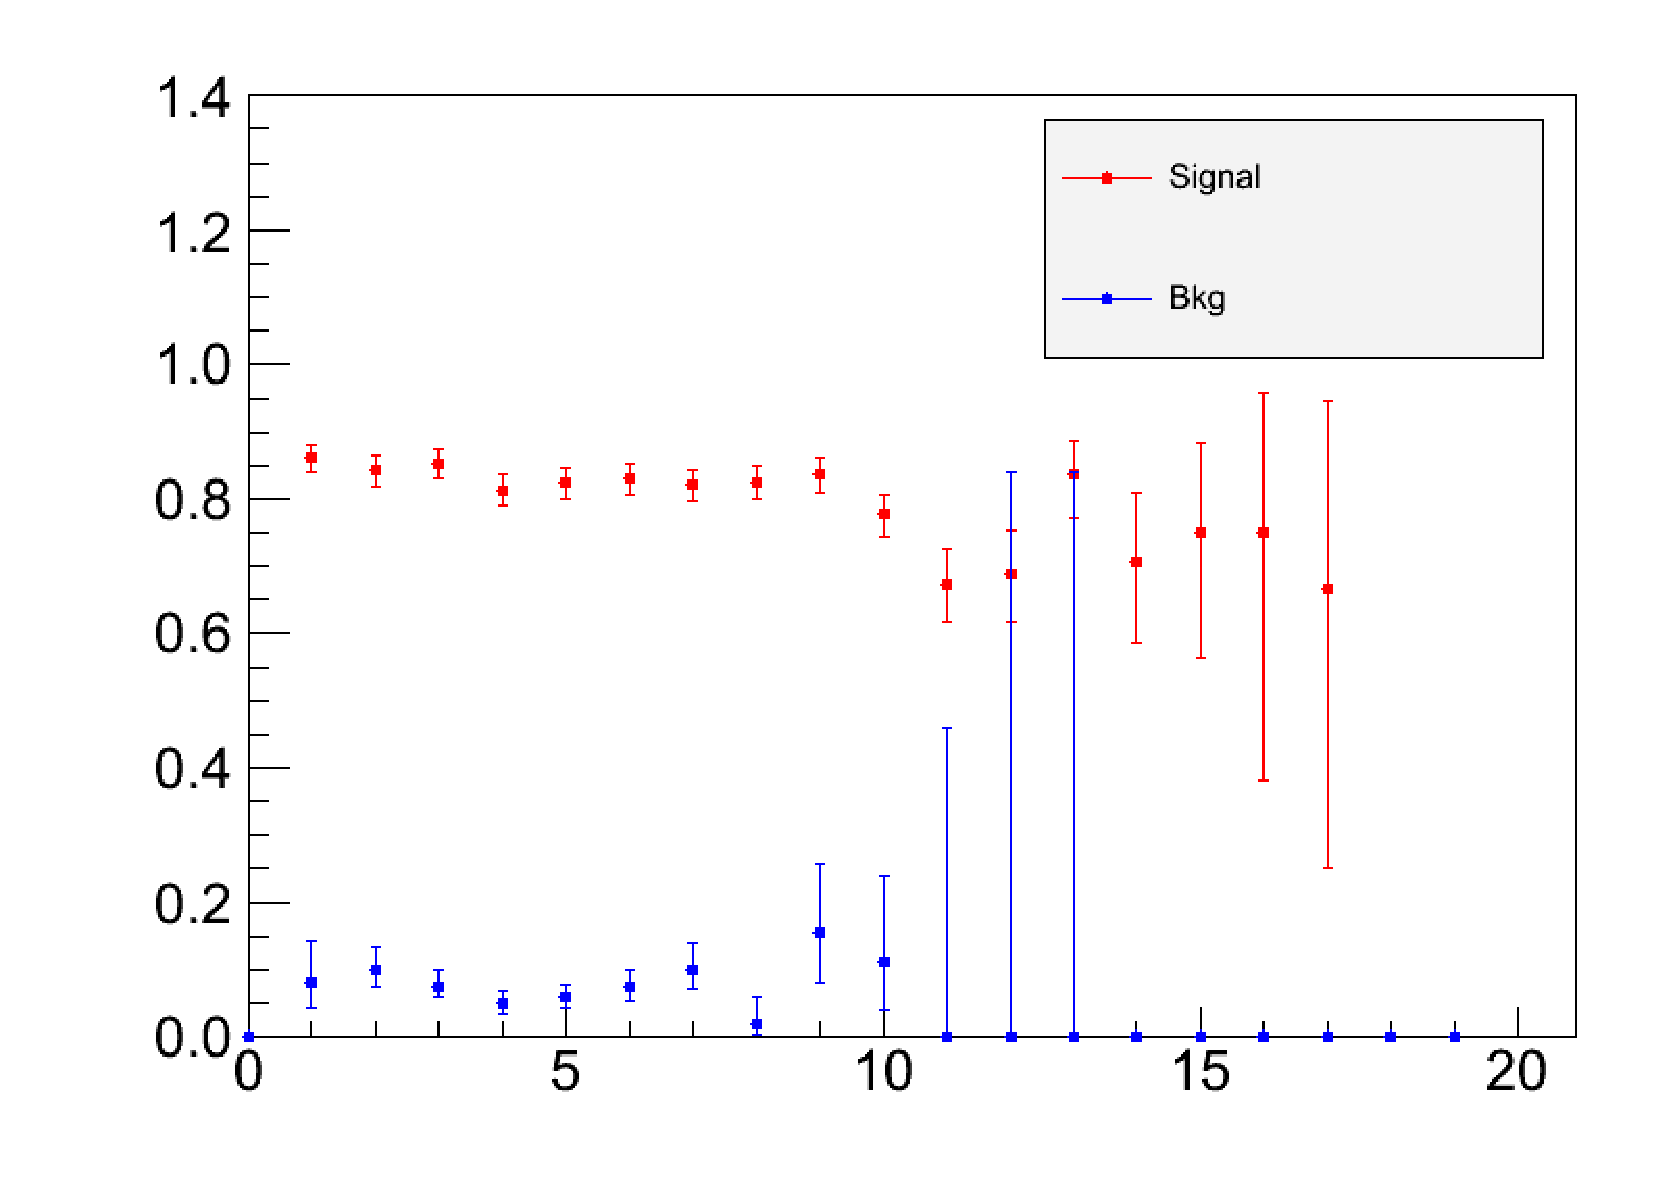
\includegraphics[width=0.48\textwidth]{figures/EleIsoEffVsNVtx_PFIso_Barrel_Pt10To15.pdf}}
\subfigure[Endcap]{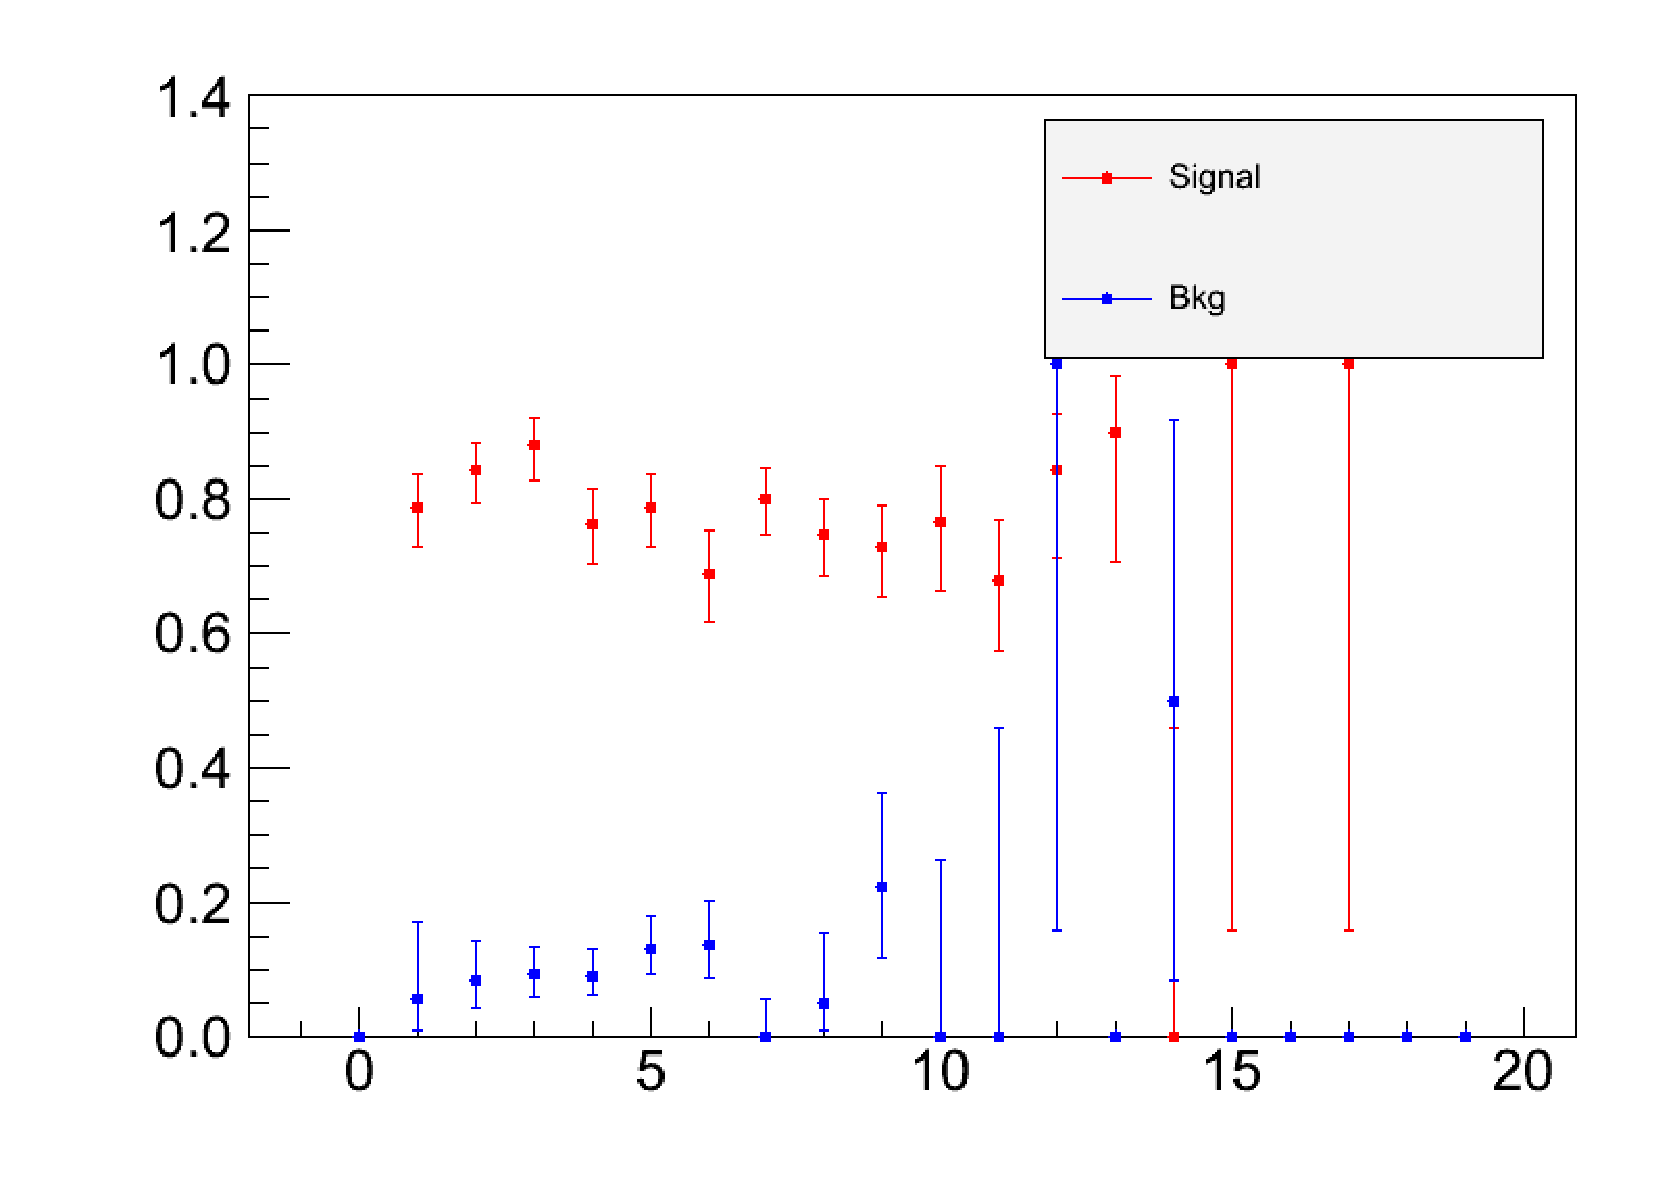
\includegraphics[width=0.48\textwidth]{figures/EleIsoEffVsNVtx_PFIso_Endcap_Pt10To15.pdf}}
\caption{The isolation efficiency of the particle flow isolation cut with the $1$GeV threshold on neutrals
for leptons with $p_{T}$ between $10$ and $15$ GeV in the HWW130 signal sample as a function of the 
number of reconstructed primary vertices, for barrel and endcap electrons.  }
\label{fig:EleIsoEffVsNVtx_PFIso_Pt10To15}
\end{center}
\end{figure}

\begin{figure}[!htbp]
\begin{center}
\subfigure[Barrel]{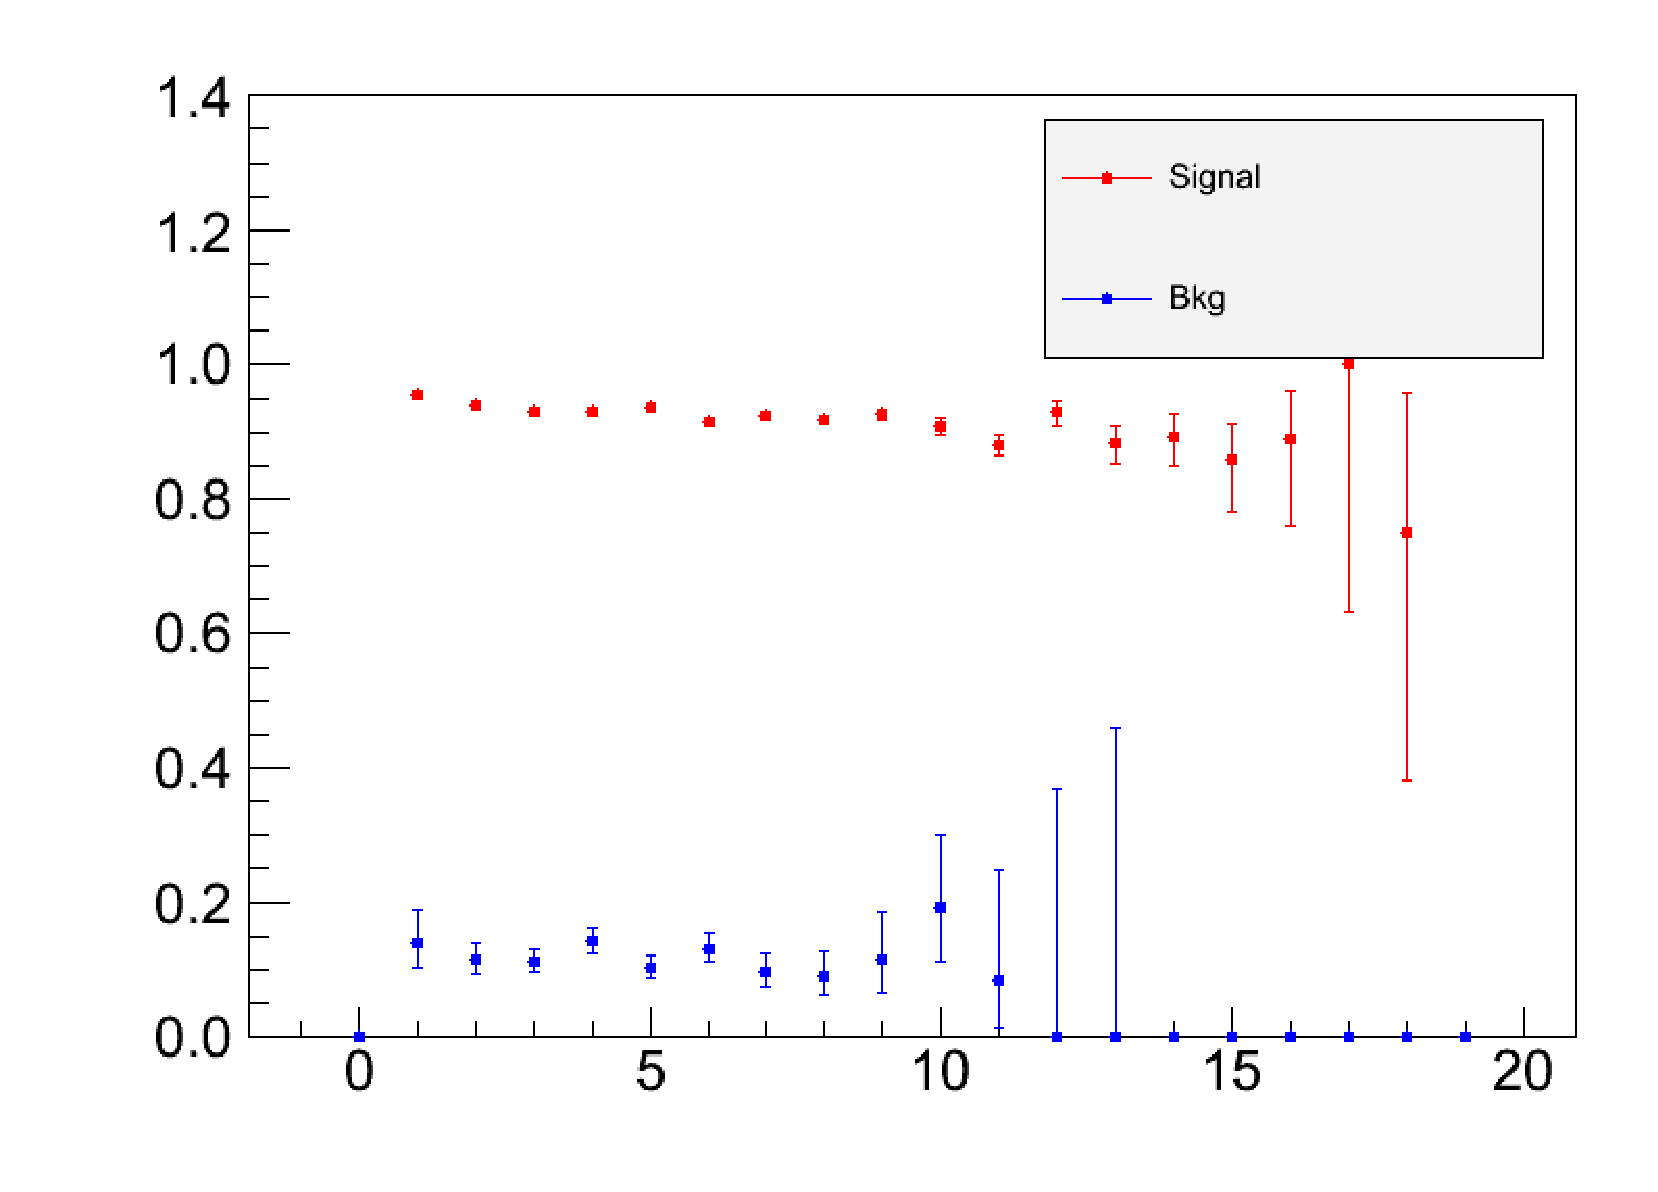
\includegraphics[width=0.48\textwidth]{figures/EleIsoEffVsNVtx_PFIso_Barrel_Pt20To30.pdf}}
\subfigure[Endcap]{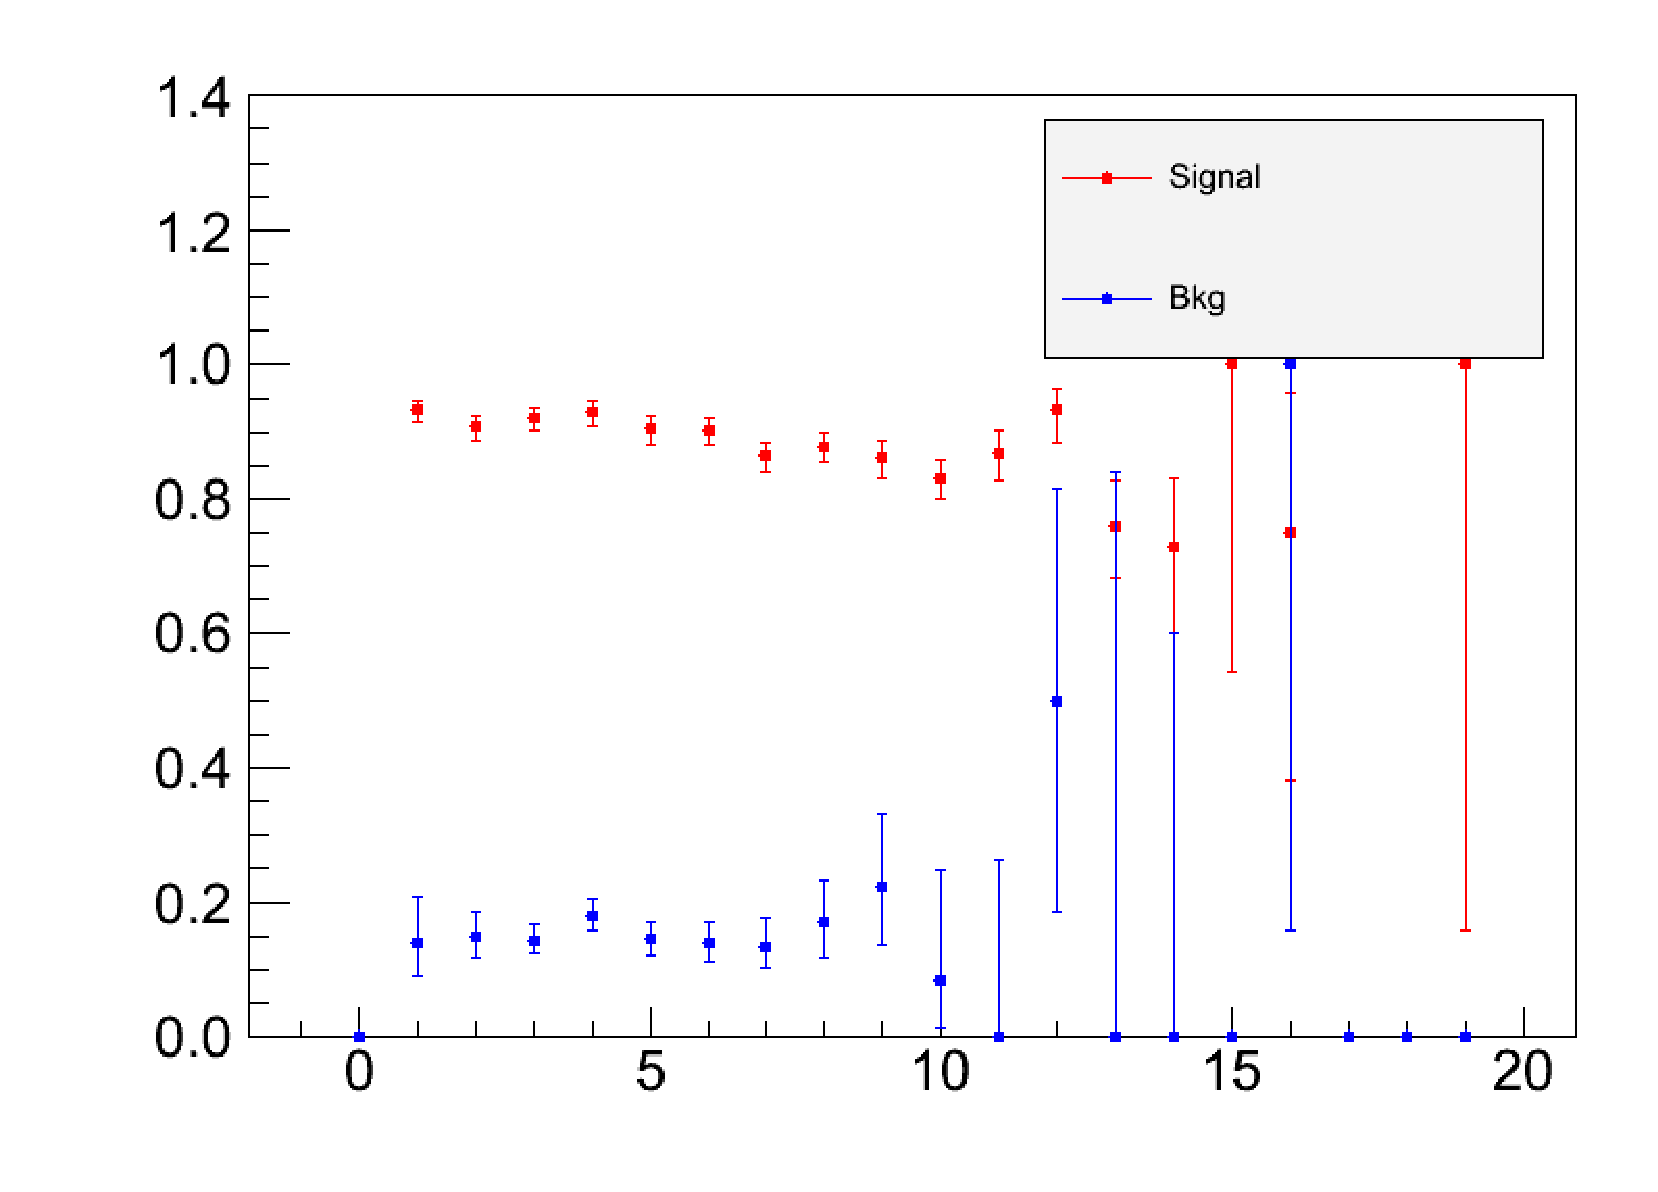
\includegraphics[width=0.48\textwidth]{figures/EleIsoEffVsNVtx_PFIso_Endcap_Pt20To30.pdf}}
\caption{The isolation efficiency of the particle flow isolation cut with the $1$GeV threshold on neutrals
for leptons with $p_{T}$ between $20$ and $30$ GeV in the HWW130 signal sample as a function of the 
number of reconstructed primary vertices, for barrel and endcap electrons.}
\label{fig:EleIsoEffVsNVtx_PFIso_Pt20To30}
\end{center}
\end{figure}

\begin{table}[!htbp]
\begin{center}
\begin{tabular}{|l|c|c|}
\hline
\multicolumn{3}{|c|}{Barrel} \\
\hline
Category                  & Std Iso Cut & PF Iso Cut \\
\hline
$p_{T}$ in $(10,15)$ GeV  &  $-22\%$    & $-10\%$    \\
$p_{T}$ in $(15,20)$ GeV  &  $-12\%$    & $-5\%$     \\
$p_{T}$ in $(20,30)$ GeV  &  $-10\%$    & $-2\%$     \\
\hline
\multicolumn{3}{|c|}{Endcap} \\
\hline
Category                  & Std Iso Cut & PF Iso Cut \\
\hline
$p_{T}$ in $(10,15)$ GeV  &  $-21\%$    & $-3\%$    \\
$p_{T}$ in $(15,20)$ GeV  &  $-6\%$    & $-1\%$     \\
$p_{T}$ in $(20,30)$ GeV  &  $-7\%$    & $-7\%$     \\

\hline
\end{tabular}
\caption{Comparison of the fractional loss of isolation efficiency for electrons from no 
pileup to a scenario with $10$ reconstructed primary vertices. }
\label{tab:EleIsoEfficiency_LossFromPileup_CompareStdWithPF}
\end{center}
\end{table}





\subsection{Isolation Algorithms Performances}

From here on, we will only compare the performance of the particle flow based isolation employing
the two different strategies for addressing pileup described in Sections 
\ref{sec:CorrectionBasedIsolation} and \ref{sec:ThresholdBasedIsolation}. 
In Figure \ref{fig:IsoPerformance_EleBarrel_BestChoices_LowPU} we compare the performance of the 
standard detector based isolation corrected with the effective area subtraction scheme with the 
two variations of PF isolation described above at the pileup 
scenario faced in the first $200$ \ipb of the 2011 data for electrons in the barrel. The working 
point for the standard detector based isolation cut from the WW  cross section measurement with 
$36$ \ipb is marked, along with three additional working points using the particle flow isolation 
with the $0.4$ cone size. We observe that for electrons with $p_{T} < 20$ GeV, there is a 
significant gain in performance for the particle flow isolation. One can gain an additional 
background rejection of $40\%$ with the same signal efficiency at low $p_{T}$. At higher $p_{T}$ 
we observe that the $1$GeV threshold on neutrals begins to hurt the performance, as well as the 
bigger size of the isolation cone. 


\begin{figure}[!htbp]
\begin{center}
\subfigure[$p_{T}$ in $(10,15)$ GeV]{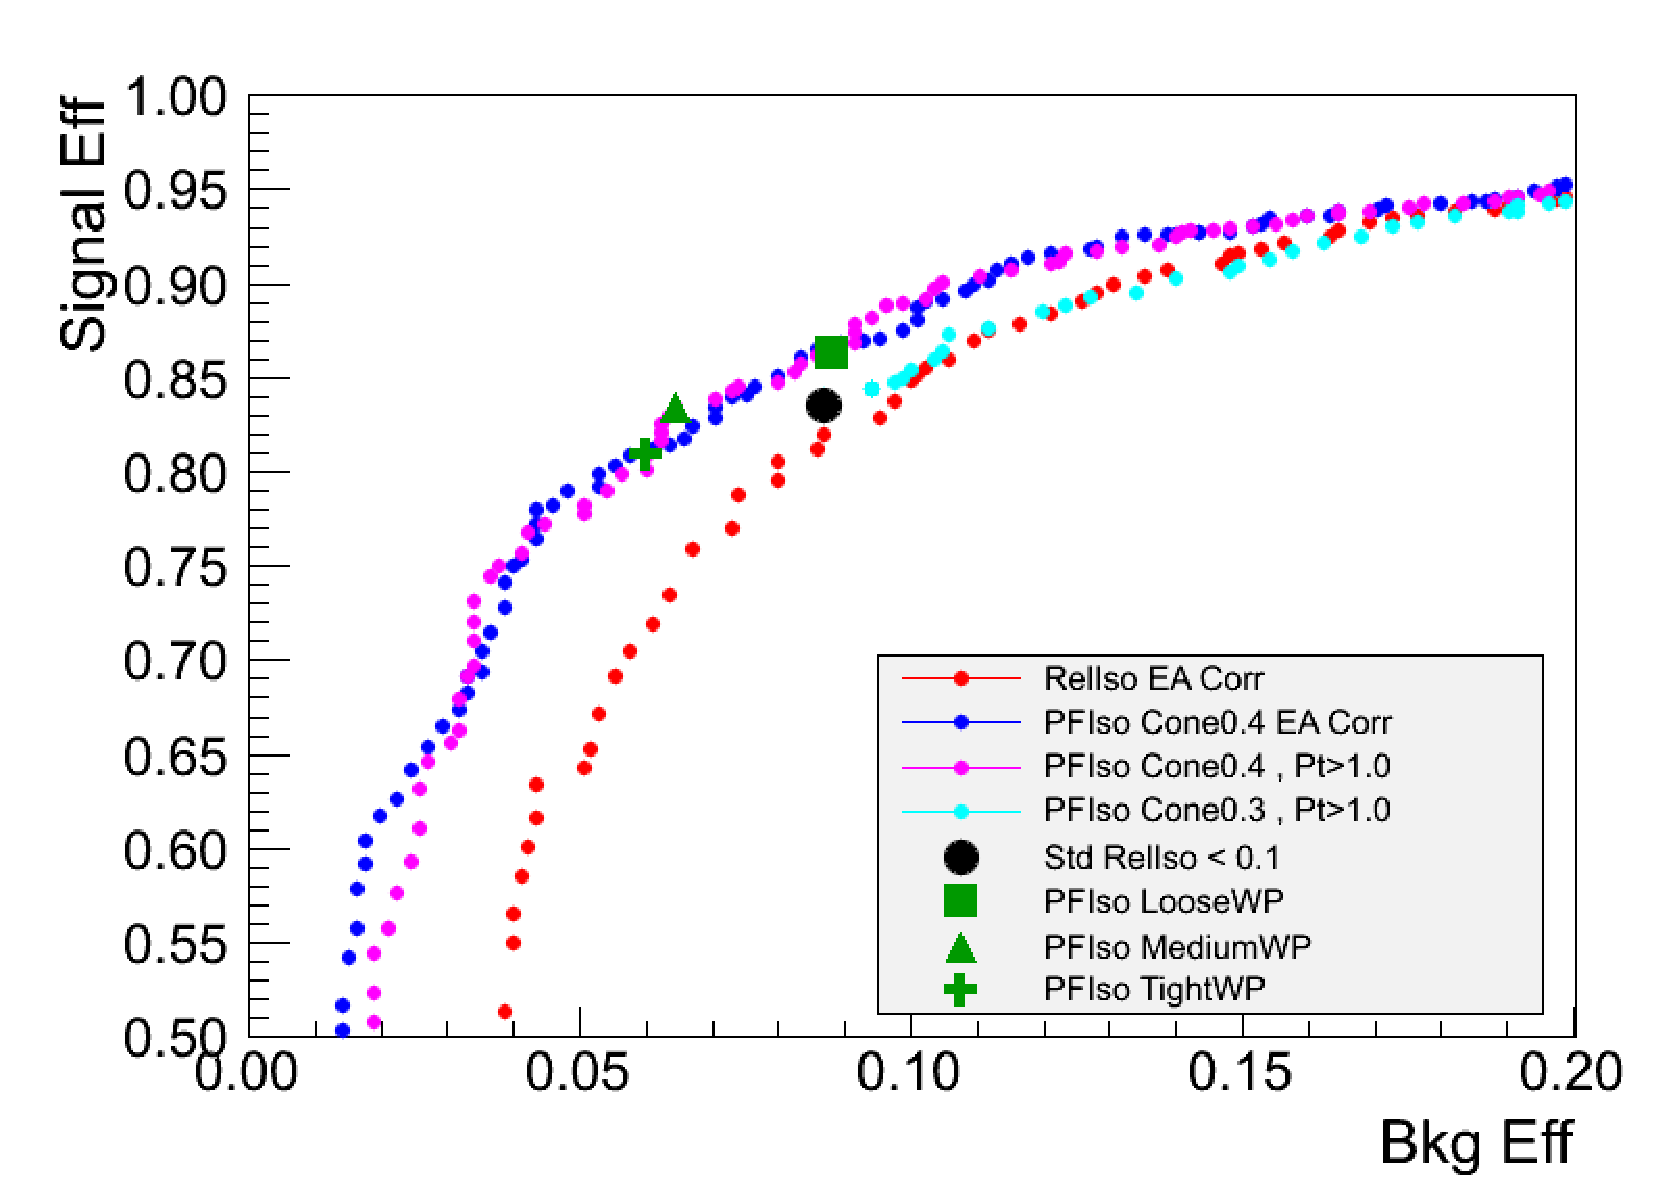
\includegraphics[width=0.48\textwidth]{figures/IsoPerformance_EleBarrel_BestChoices_NVtx3To6_Pt10To15.pdf}}
\subfigure[$p_{T}$ in $(15,20)$ GeV]{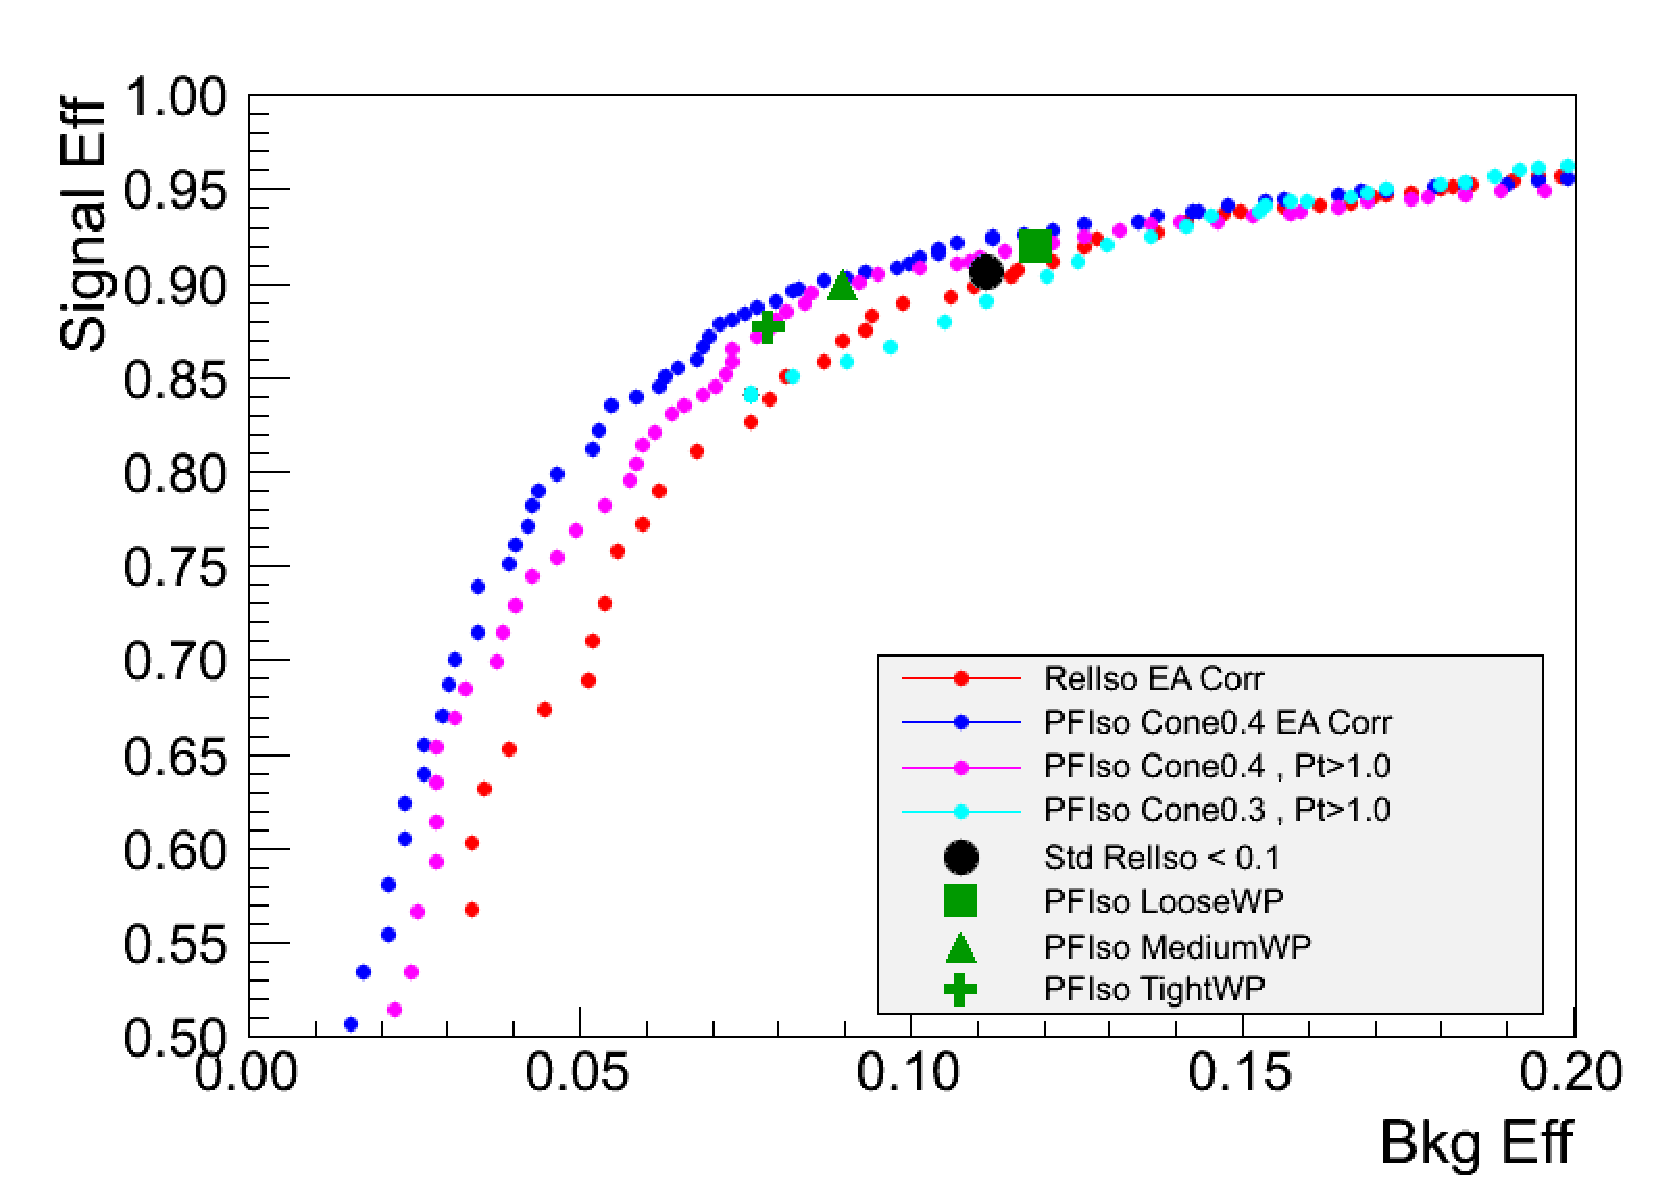
\includegraphics[width=0.48\textwidth]{figures/IsoPerformance_EleBarrel_BestChoices_NVtx3To6_Pt15To20.pdf}}
\subfigure[$p_{T}$ in $(20,30)$ GeV]{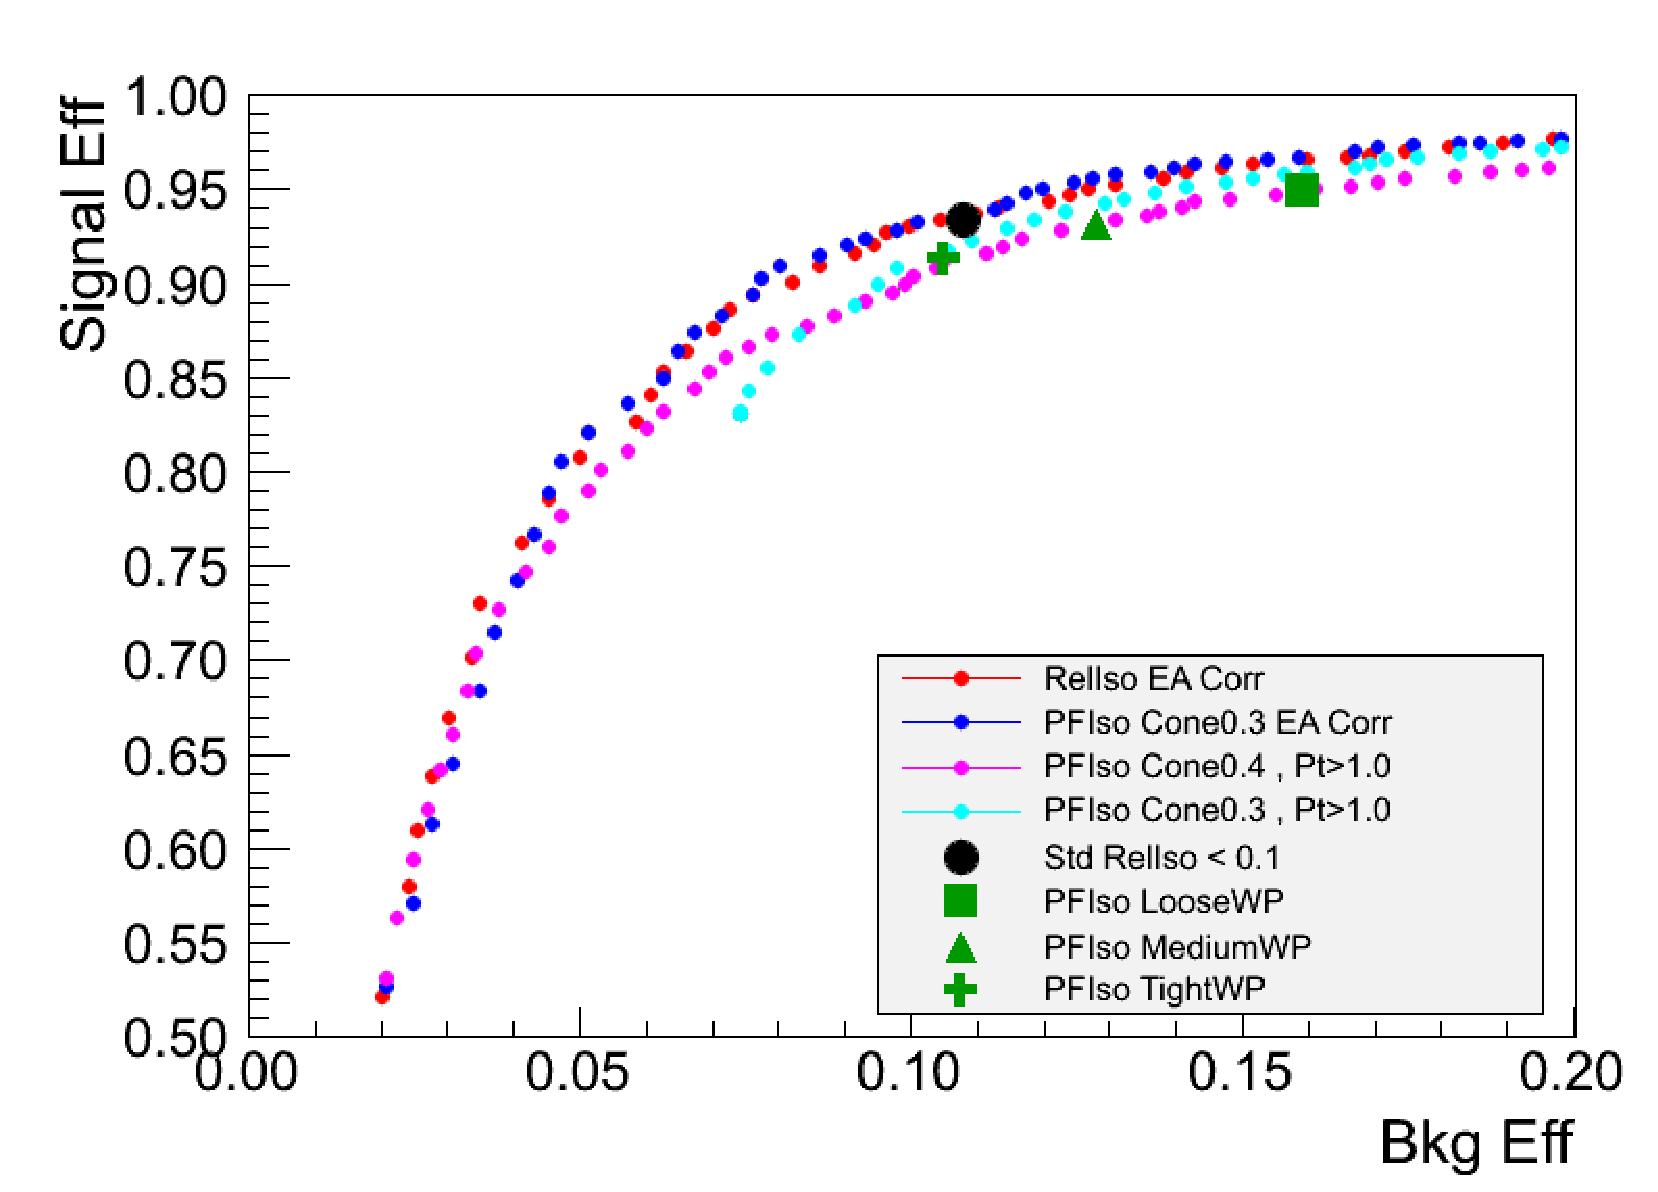
\includegraphics[width=0.48\textwidth]{figures/IsoPerformance_EleBarrel_BestChoicesCone03_NVtx3To6_Pt20To30.pdf}}
\caption{ Signal efficiency (HWW130) vs background efficiency for barrel electrons at low pileup, 
separated into different $p_{T}$ bins, comparing the standard isolation with the best choices .
we have for the particle flow isolation.}
\label{fig:IsoPerformance_EleBarrel_BestChoices_LowPU}
\end{center}
\end{figure}

\clearpage

In Figure \ref{fig:IsoPerformance_EleEndcap_BestChoices_LowPU}, we make the same comparison for 
electrons in the endcap. In the endcap, we observe the the $1$ GeV threshold is degrading the 
performance more than in the barrel. For high $p_{T}$, the smaller cone size, again,
gives the best performance. 


\begin{figure}[!htbp]
\begin{center}
\subfigure[$p_{T}$ in $(10,15)$ GeV]{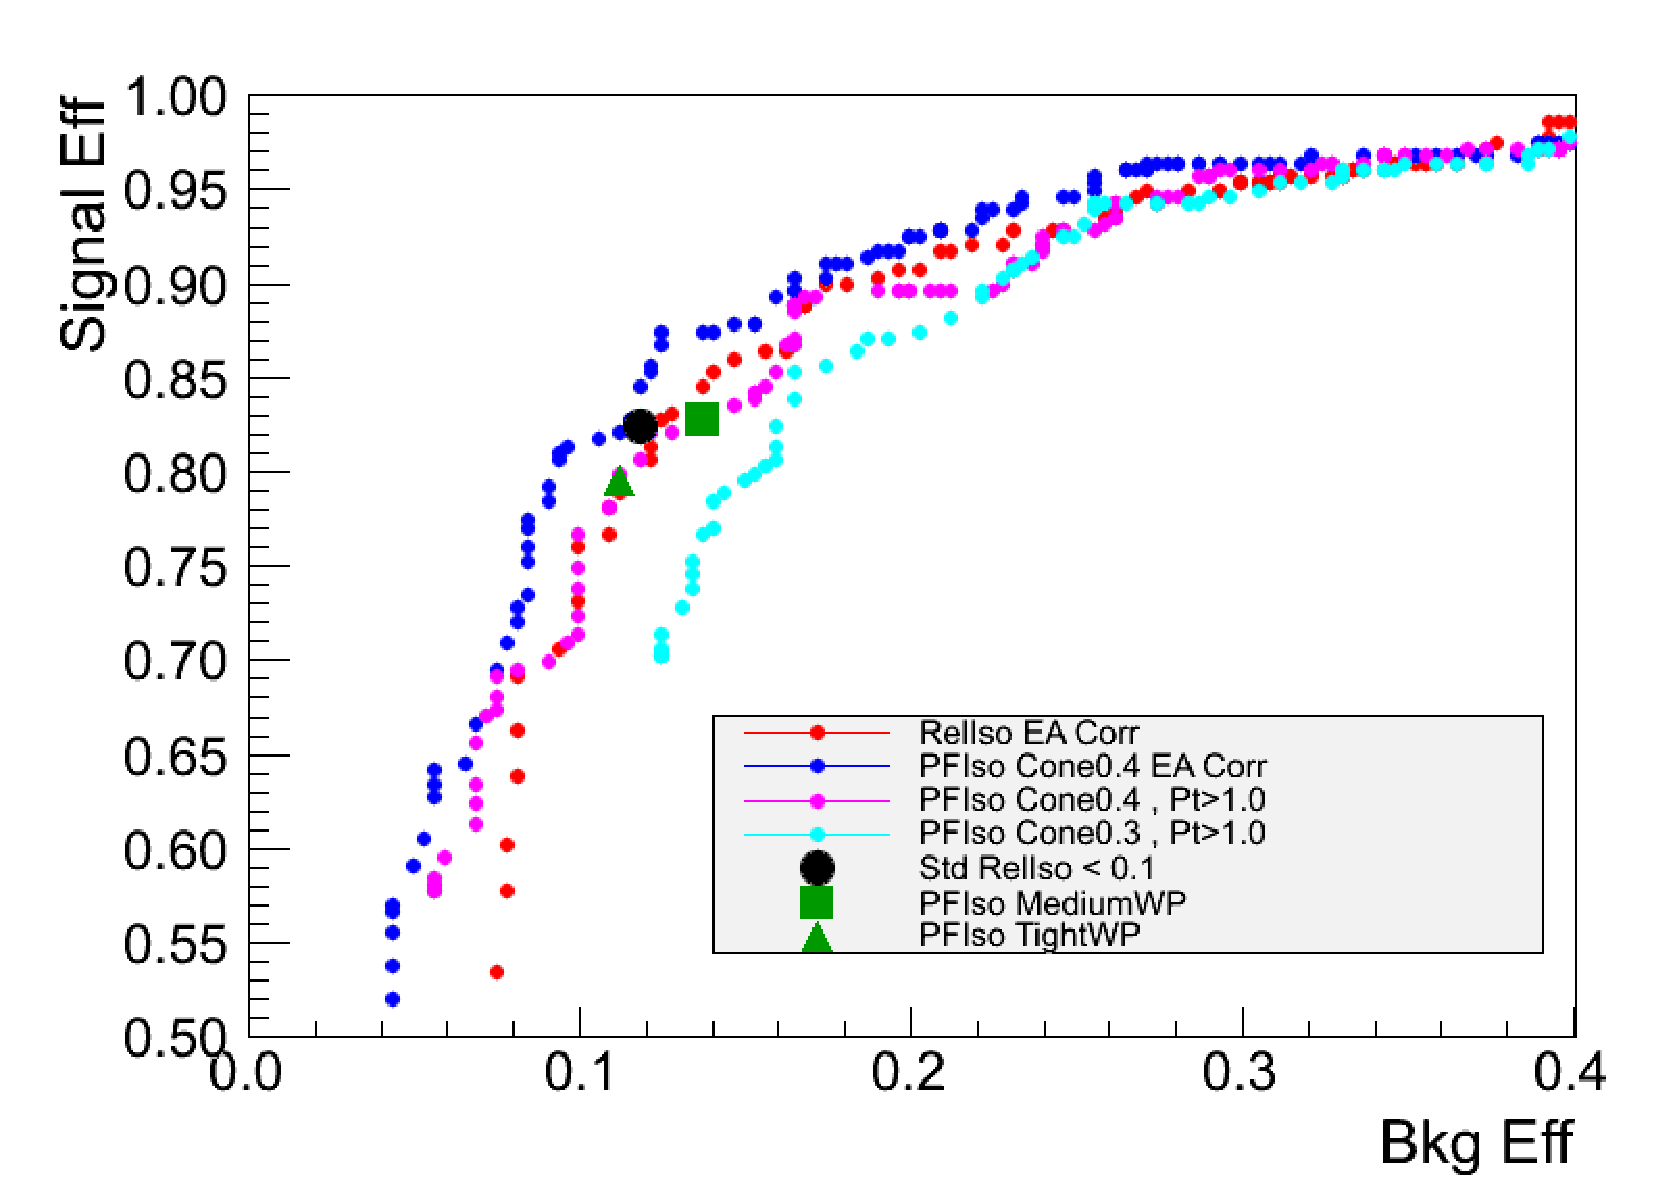
\includegraphics[width=0.48\textwidth]{figures/IsoPerformance_EleEndcap_BestChoices_NVtx3To6_Pt10To15.pdf}}
\subfigure[$p_{T}$ in $(15,20)$ GeV]{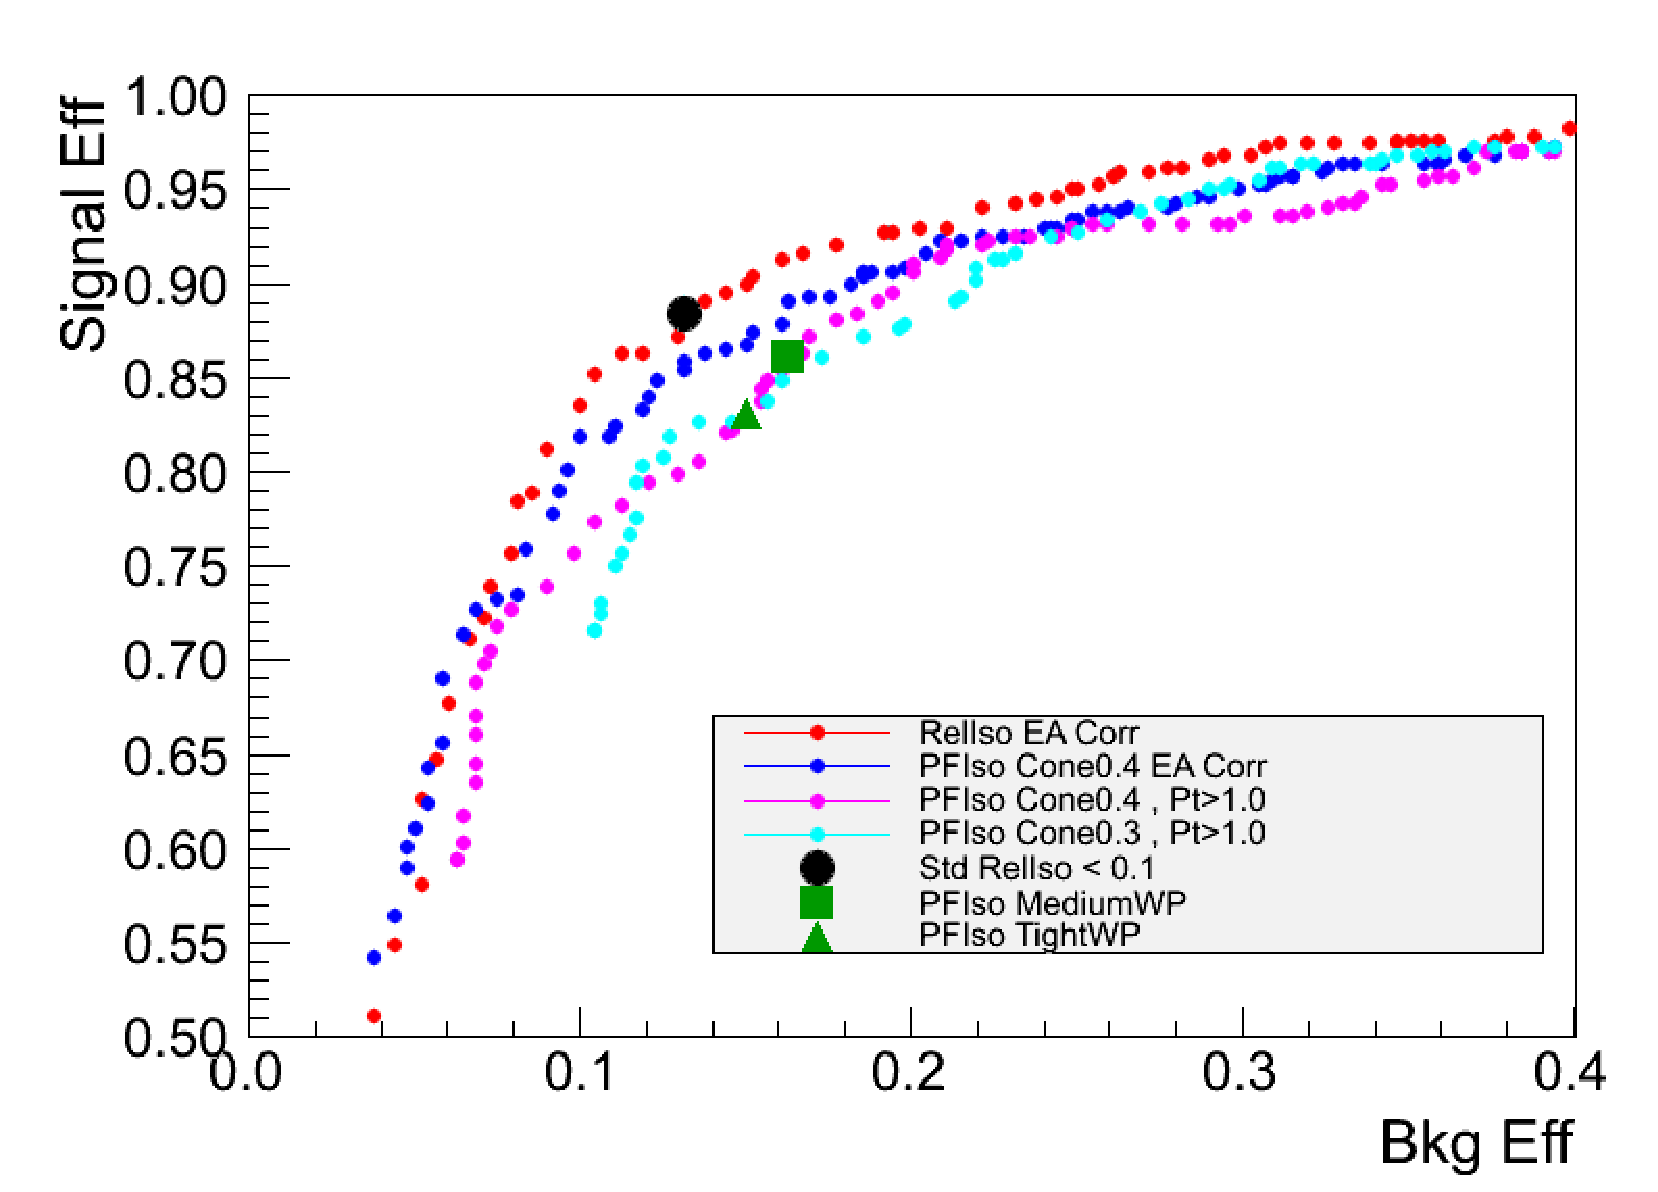
\includegraphics[width=0.48\textwidth]{figures/IsoPerformance_EleEndcap_BestChoices_NVtx3To6_Pt15To20.pdf}}
\subfigure[$p_{T}$ in $(20,30)$ GeV]{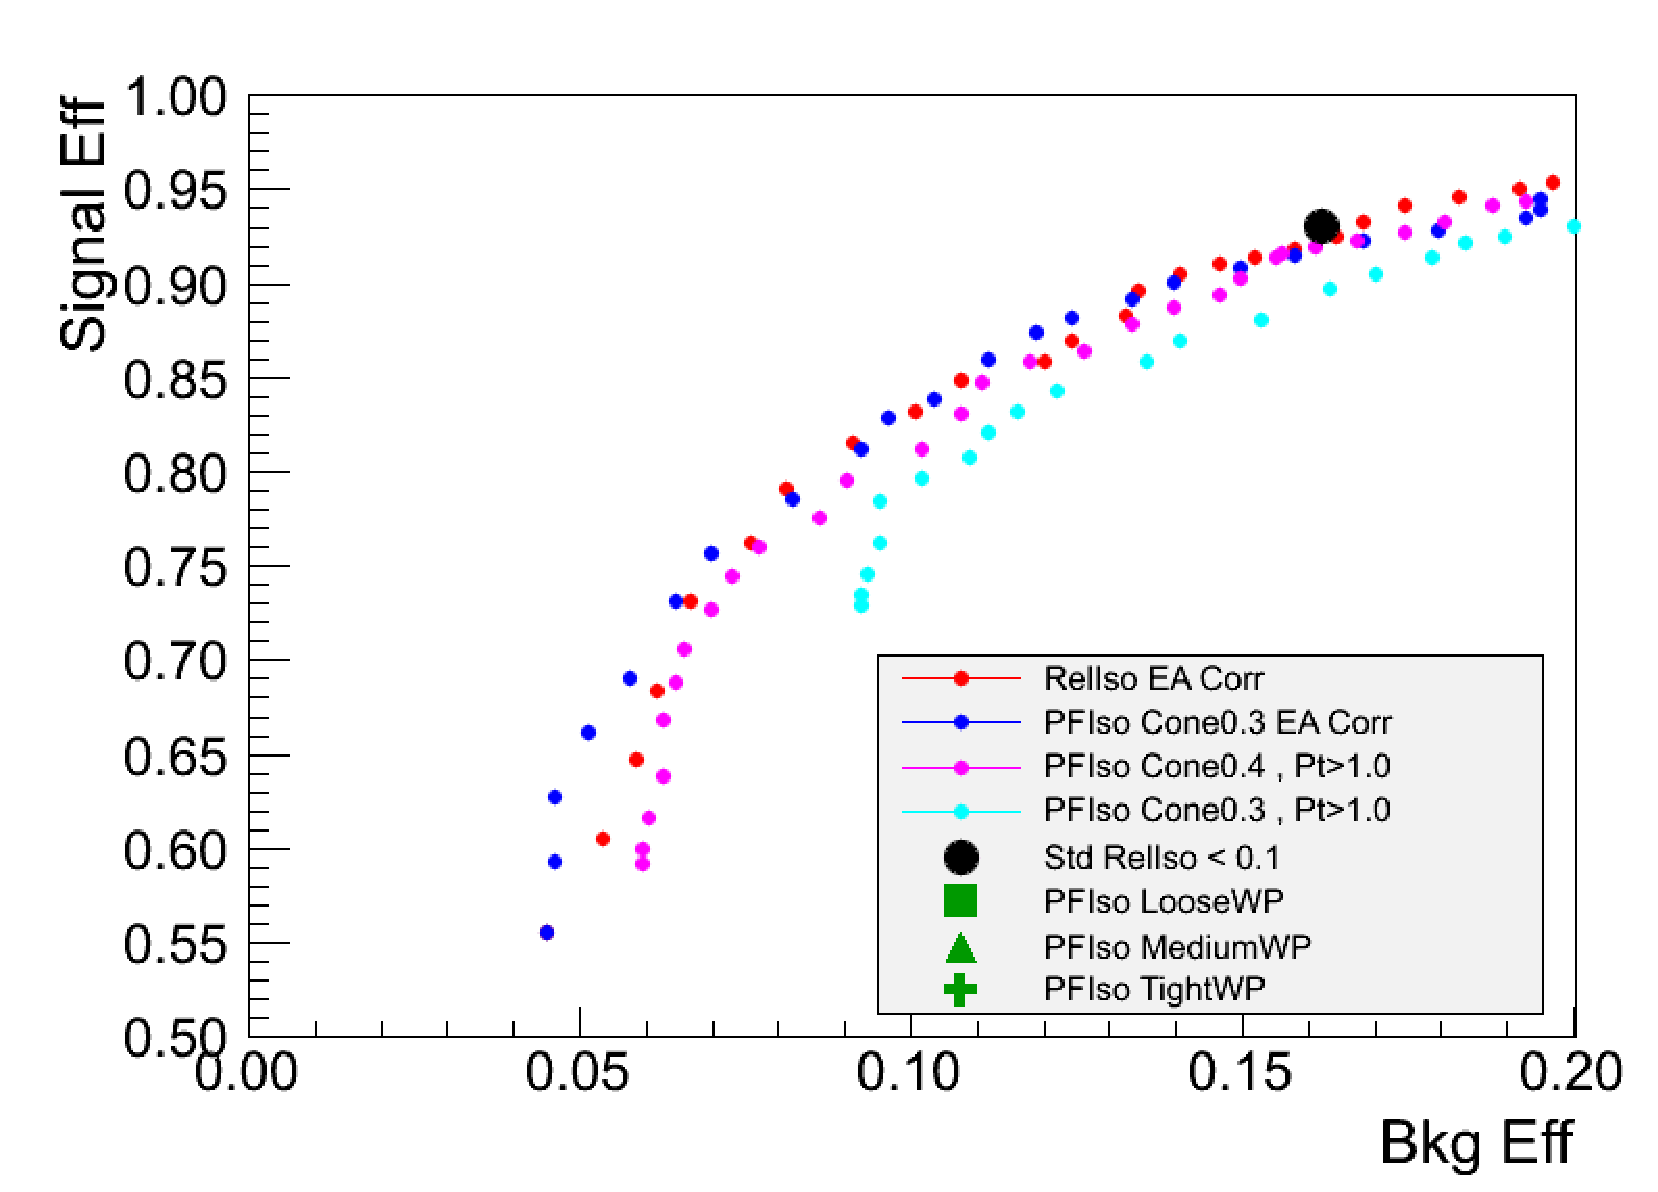
\includegraphics[width=0.48\textwidth]{figures/IsoPerformance_EleEndcap_BestChoicesCone03_NVtx3To6_Pt20To30.pdf}}
\caption{Signal efficiency (HWW130) vs background efficiency for endcap electrons at low pileup
separated into different $p_{T}$ bins, comparing the standard isolation with the best choices .
we have for the particle flow isolation.}
\label{fig:IsoPerformance_EleEndcap_BestChoices_LowPU}
\end{center}
\end{figure}

\clearpage

In Figure \ref{fig:IsoPerformance_EleBarrel_BestChoices_HighPU}, we make the same comparison again for the
barrel but with a much more severe pileup scenario, selecting events with the number of reconstructed
vertices between $7$ and $15$. At high pileup, we observe a huge gain in performance for the particle
flow isolation relative to the detector based isolation. At higher $p_{T}$ we are again being 
adversely affected by the $1$ GeV threshold, and to a lesser degree the larger cone size. 




\begin{figure}[!htbp]
\begin{center}
\subfigure[$p_{T}$ in $(10,15)$ GeV]{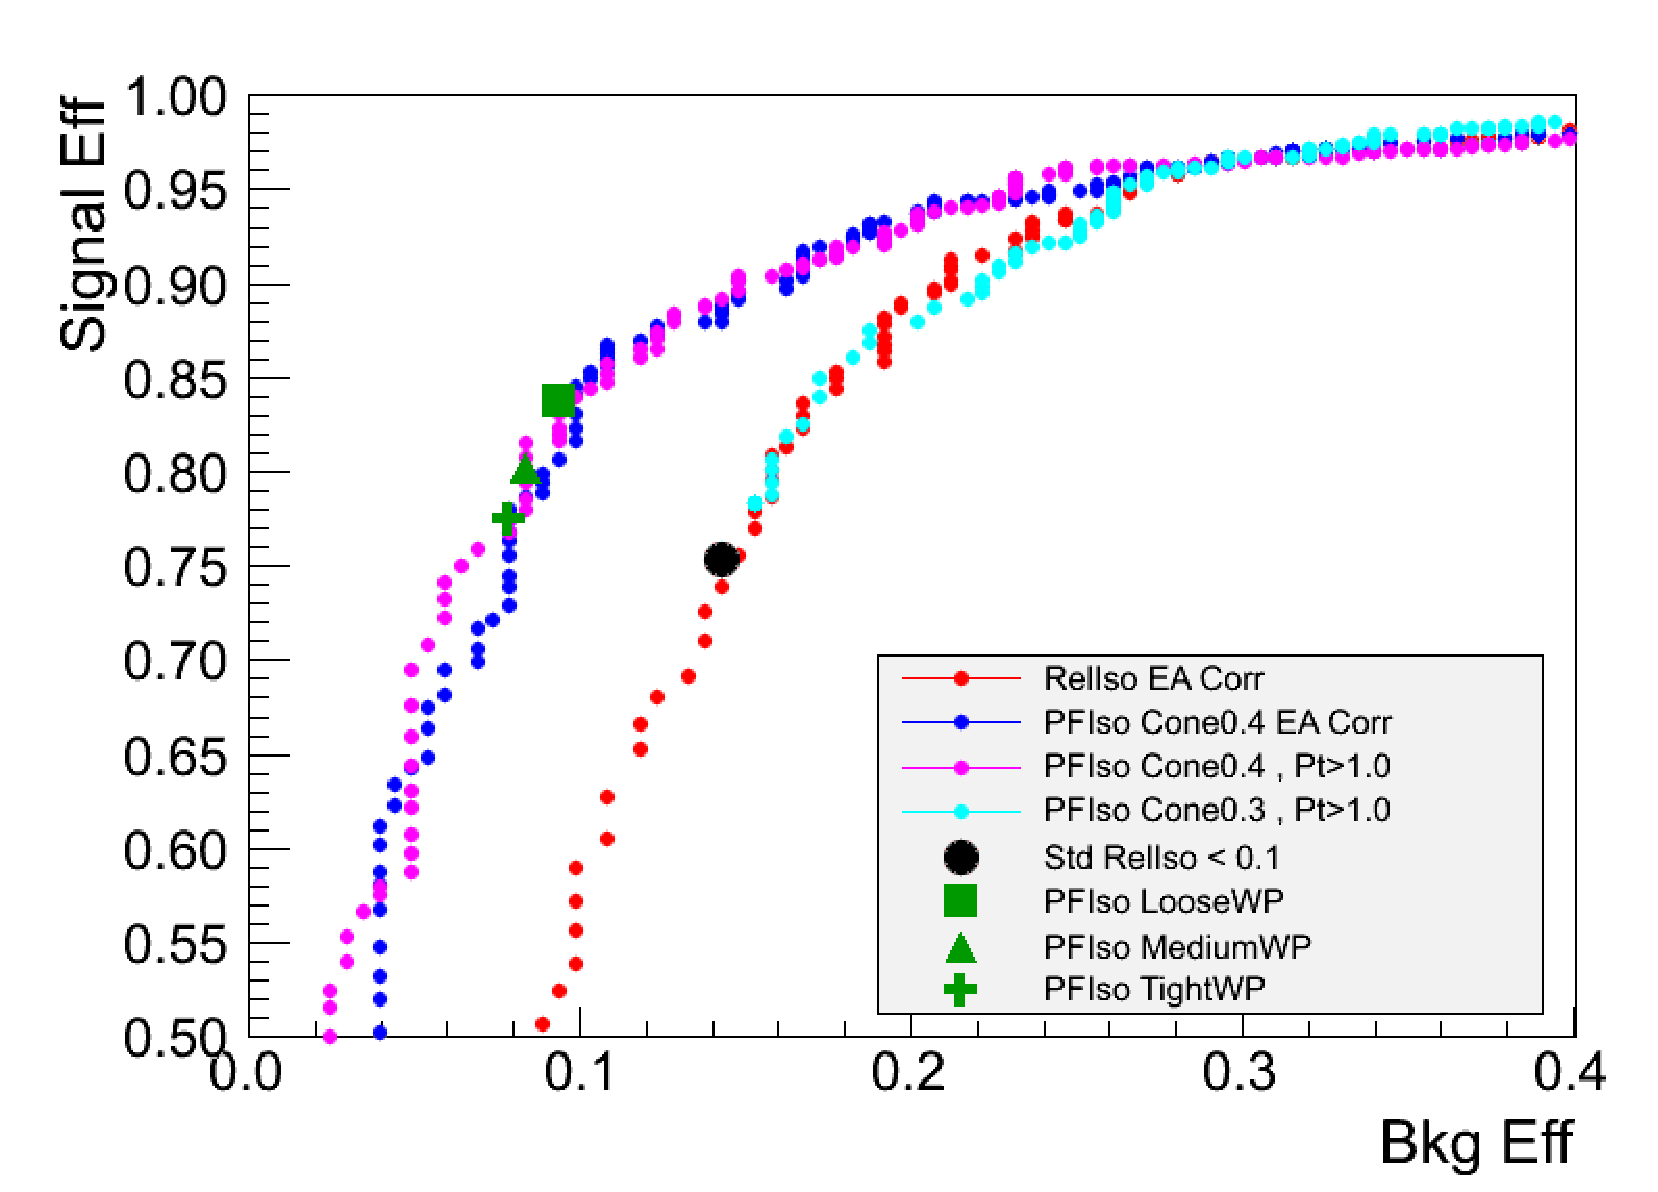
\includegraphics[width=0.48\textwidth]{figures/IsoPerformance_EleBarrel_BestChoices_NVtx7To15_Pt10To15.pdf}}
\subfigure[$p_{T}$ in $(15,20)$ GeV]{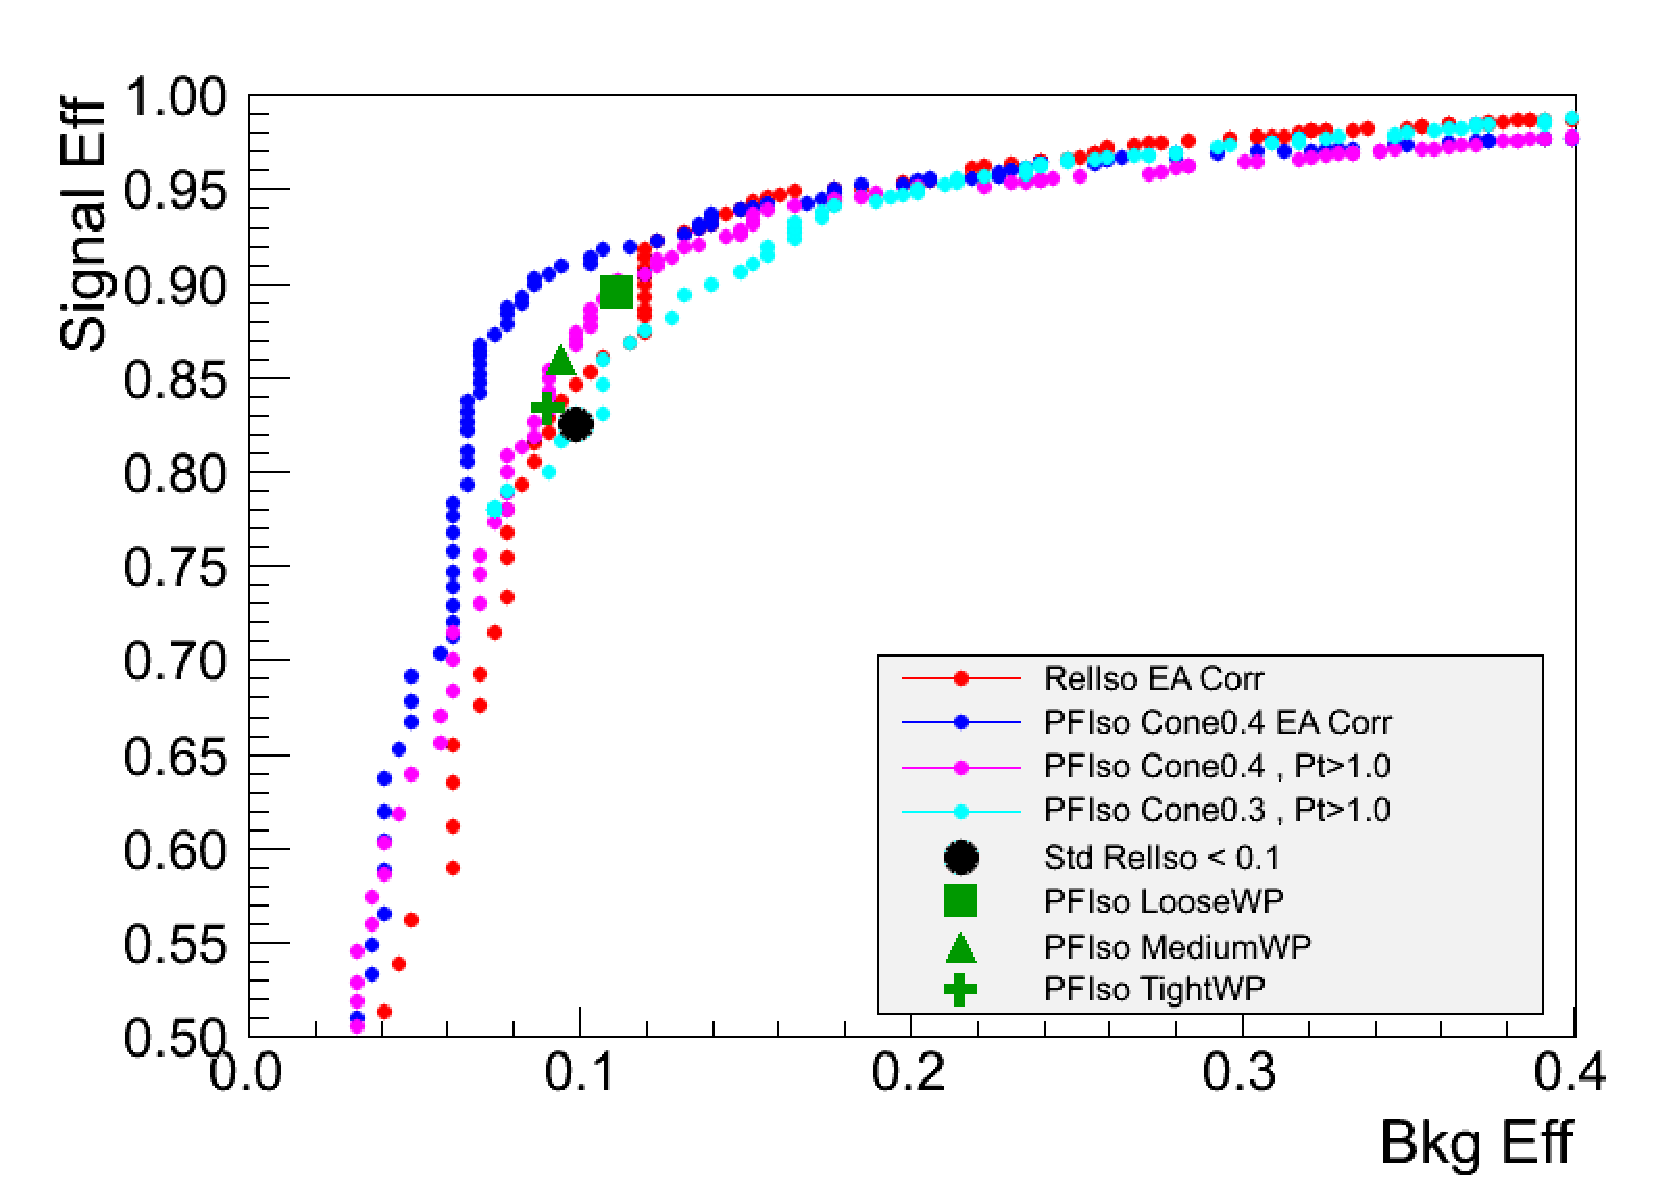
\includegraphics[width=0.48\textwidth]{figures/IsoPerformance_EleBarrel_BestChoices_NVtx7To15_Pt15To20.pdf}}
\subfigure[$p_{T}$ in $(20,30)$ GeV]{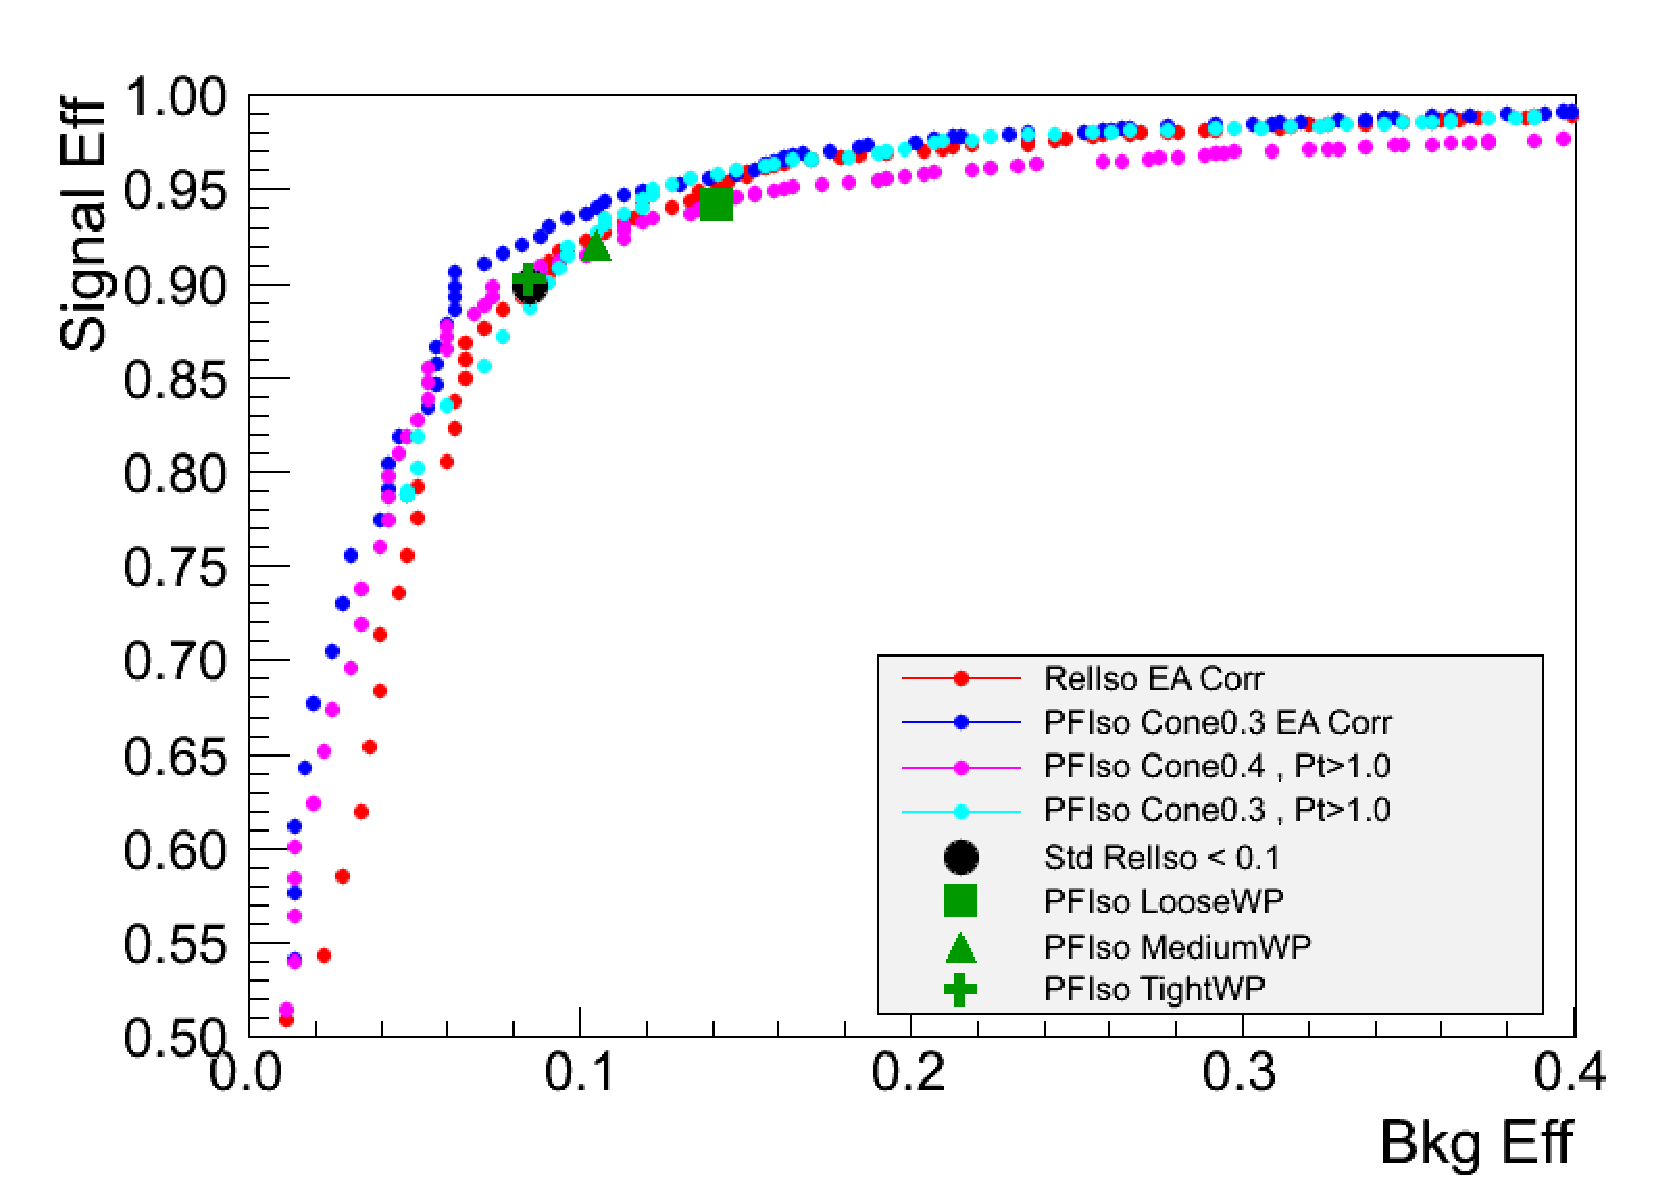
\includegraphics[width=0.48\textwidth]{figures/IsoPerformance_EleBarrel_BestChoicesCone03_NVtx7To15_Pt20To30.pdf}}
\caption{Signal efficiency (HWW130) vs background efficiency for barrel electrons at high pileup
separated into different $p_{T}$ bins, comparing the standard isolation with the best choices .
we have for the particle flow isolation.}
\label{fig:IsoPerformance_EleBarrel_BestChoices_HighPU}
\end{center}
\end{figure}

\clearpage

In Figure \ref{fig:IsoPerformance_EleEndcap_BestChoices_HighPU}, we perform the same comparison for
the endcap at high pileup. Here we suffer from limited statistics in the background estimate
due to the fact that in the first $200$ \ipb of data in 2011, we did not have many events with
such high pileup conditions. Similar general trends can still be observed, however. At higher
$p_{T}$ we observe some degradation in performance due to the $1GeV$ threshold on neutrals, 
and also the larger cone size. 

\begin{figure}[!htbp]
\begin{center}
\subfigure[$p_{T}$ in $(10,15)$ GeV]{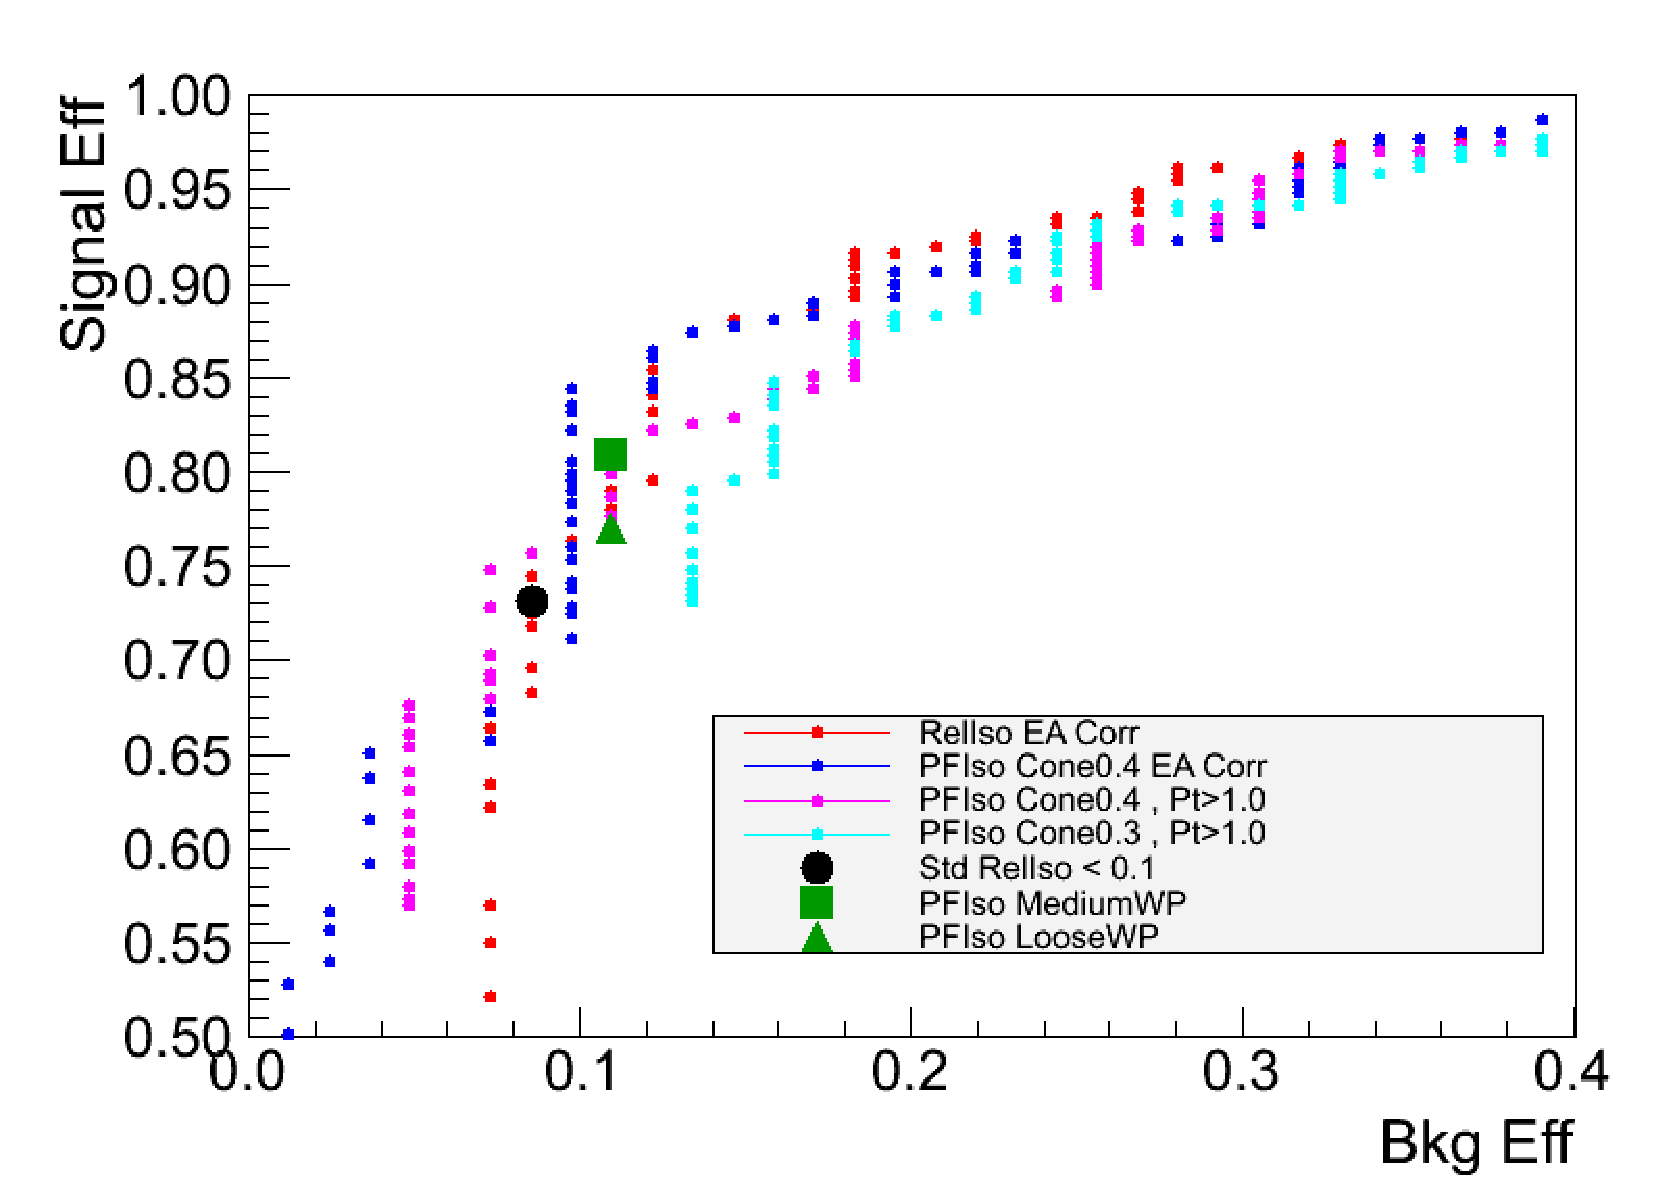
\includegraphics[width=0.48\textwidth]{figures/IsoPerformance_EleEndcap_BestChoices_NVtx7To15_Pt10To15.pdf}}
\subfigure[$p_{T}$ in $(15,20)$ GeV]{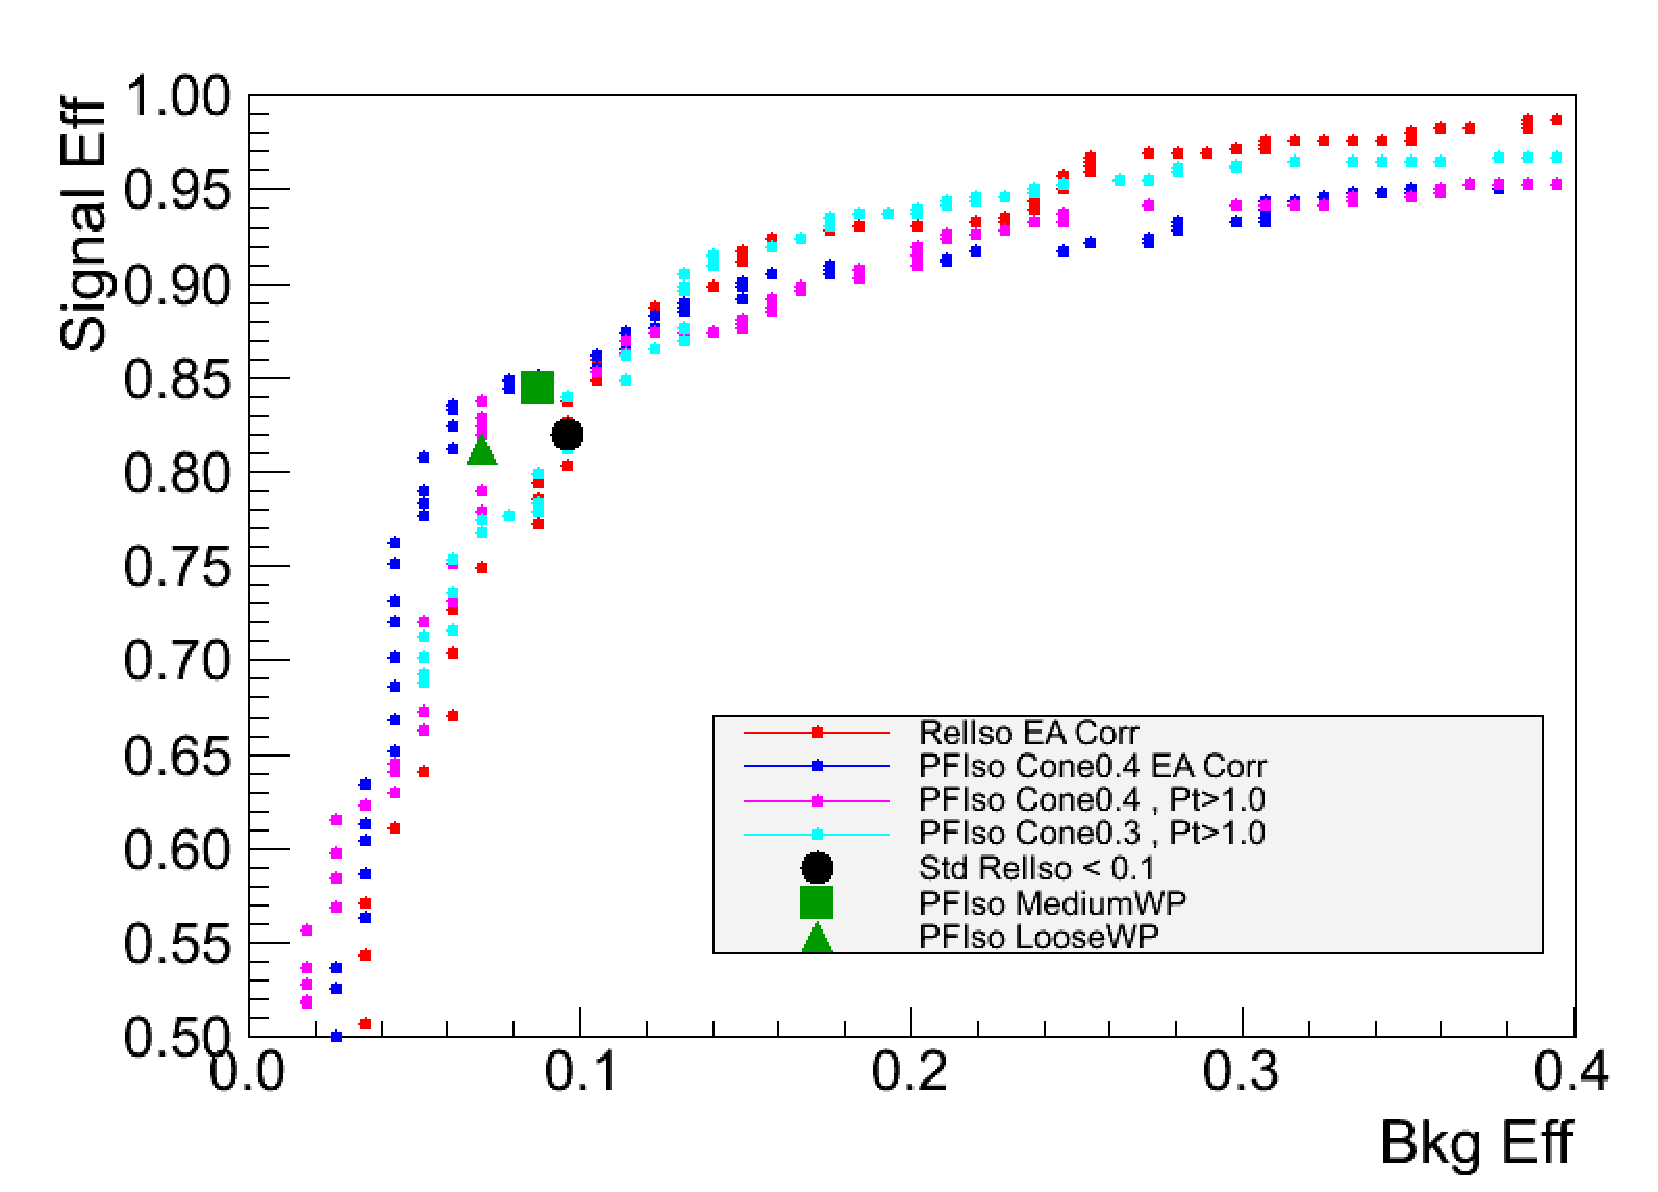
\includegraphics[width=0.48\textwidth]{figures/IsoPerformance_EleEndcap_BestChoices_NVtx7To15_Pt15To20.pdf}}
\subfigure[$p_{T}$ in $(20,30)$ GeV]{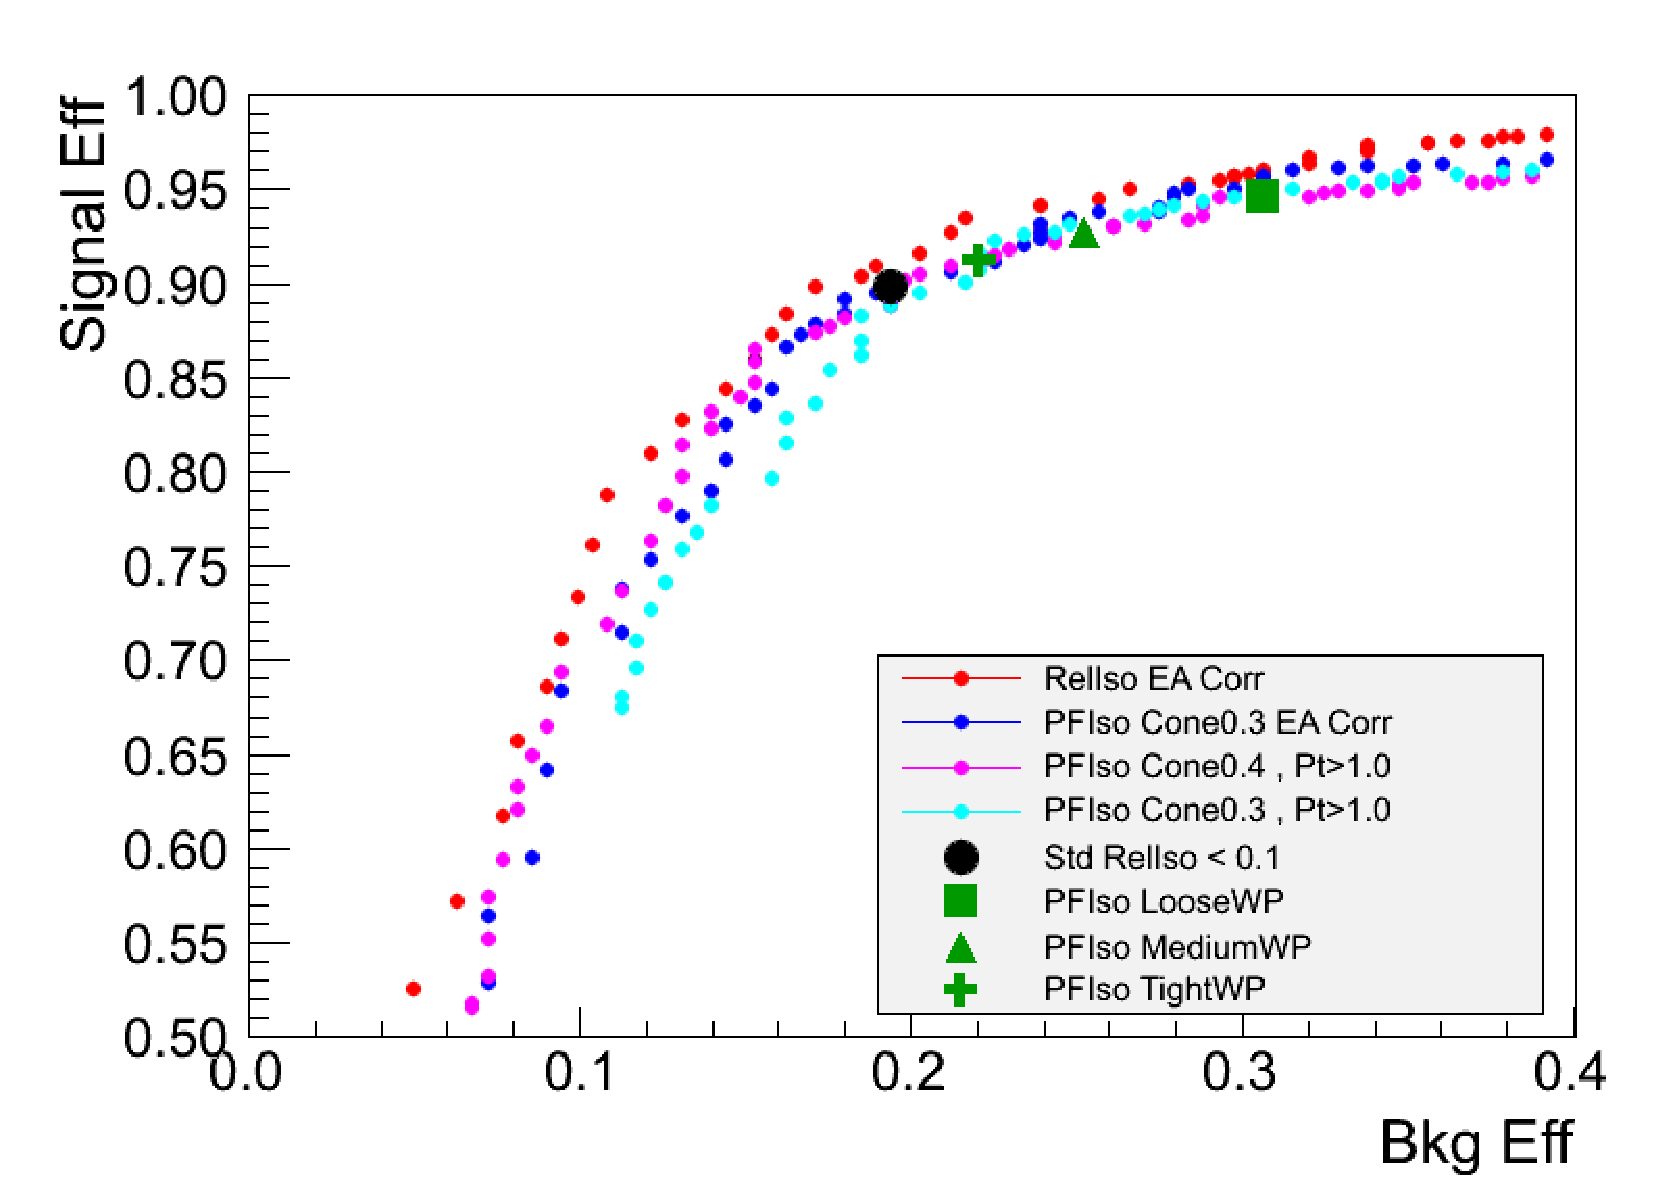
\includegraphics[width=0.48\textwidth]{figures/IsoPerformance_EleEndcap_BestChoicesCone03_NVtx7To15_Pt20To30.pdf}}
\caption{Signal efficiency (HWW130) vs background efficiency for endcap electrons at high pileup
separated into different $p_{T}$ bins, comparing the standard isolation with the best choices .
we have for the particle flow isolation.}
\label{fig:IsoPerformance_EleEndcap_BestChoices_HighPU}
\end{center}
\end{figure}

\clearpage


\subsection{Working Point Definition}

For the current analysis, we employ the threshold-based solution to mitigating the effect of pileup,
primarily for its simplicity. To obtain the best working point in terms of the actual isolation
cut values that we will use, we compare the change in the signal yield, estimated from signal
Monte Carlo, and the change in the background yield, estimated using the fake rate method,
relative to the old isolation requirement using detector-based isolation cuts. We define a number
of working points closest to the previous working point using the detector-based isolation in
signal efficiency and background efficiency, and evaluate its performance in terms of the
expected limits at $1$ \ifb. This optimization procedure has been performed primarily focusing on
low mass higgs signal ($m_{\mathrm{H}} <= 130$ GeV ). 

The working point we arrived at is summarized in Table \ref{tab:PFIsoWorkingPoint}. For muons, an isolation cone of
$0.3$ is used, where we observe that the loss of efficiency due to the two leptons from the
W decay being within $\Delta$ R $ < 0.4$ has significant impact on performance. For electrons, an
isolation cone of $0.4$ is used, where we observe that the extra gain in background rejection
at low $p_{T}$ resulting from the bigger cone size has a very important positive impact on 
performance. The different cuts for barrel and endcap, and low and high $p_{T}$ have been tuned
primarily to achieve fake rates that are relatively close to the old detector-based
isolation working point.

\begin{table}[!htbp]
\begin{center}
\begin{tabular}{|l|c|c|}
\hline
\multicolumn{3}{|c|}{Electrons} \\
\hline
$p_{T}$ Bin      & Barrel $(\eta_{\mathrm{supercluster}} < 1.479$) & Endcap $(\eta_{\mathrm{supercluster}} >= 1.479$) \\
\hline
$(10,20)$ GeV  &  $0.06$    & $0.05$     \\
$(20+)$ GeV    &  $0.13$    & $0.09$     \\
\hline
\multicolumn{3}{|c|}{Muons} \\
\hline
$p_{T}$ Bin      & Barrel $(\eta < 1.479$) & Endcap $(\eta >= 1.479$) \\

\hline
$(10,20)$ GeV  &  $0.13$    & $0.09$     \\
$(20+)$ GeV    &  $0.13$    & $0.09$     \\

\hline
\end{tabular}
\caption{Cut values for the particle flow isolation in bins of $p_{T}$ and $\eta$ for electrons
and muons.  }
\label{tab:PFIsoWorkingPoint}
\end{center}
\end{table}

The highlight of using this isolation working point is that it allows us to include electrons 
with $p_{T}$ between $10$ and $15$ GeV, without increasing the total fake lepton background
yield. For a higgs signal with mass of $130$ GeV, we gain roughly $5\%$ of signal with a 
corresponding improvement in the expected limit of $5\%$. 

\subsubsection{Options for very high PU}

For the second half of 2011, there's a possiblity for the LHC to deliver a pileup scenario
that is much more severe than the scenario that was studied in this section. For such a 
scenario, we still have the option of employing the energy density based pileup 
correction which will yield flat isolation efficiencies beyond $25$ reconstructed 
vertices.

